\part{Symmetric Group Representations}
\chapter{Representation Theory of the Symmetric Group}
\label{chap:reps of Sn}
\section{Combinatoric Preliminaries}
The representation theory of the symmetric group, \(S_n\), is mostly controlled by the combinatorics of partitions.
In this section we set up some of the important objects which allow for efficient computations with representations of \(S_n\).

\begin{dfn}{Partition}{}
    Let \(n\) be a nonnegative integer.
    A \defineindex{partition} of \(n\) is a nonincreasing sequence of nonnegative integers, \(\lambda = (\lambda_1, \lambda_2, \lambda_3, \dotsc)\), such that \(\lambda_1 + \lambda_2 + \lambda_3 + \dotsb = n\).
\end{dfn}

\begin{ntn}{}{}
    We write \(\lambda \partition n\) to say that \(\lambda\) is a partition of \(n\).
    
    We write \(\abs{\lambda}\) for \(n\).
    
    We write \(\ell(\lambda)\) for the number of nonzero parts, that is \(\lambda_\ell\) is the last nonzero term in the sequence \(\lambda\).
\end{ntn}

Notice that since \(n\) is finite and \(\lambda\) is nonincreasing it must be that \(\lambda_i = 0\) for \(i\) sufficiently large, so usually we'll just consider \(\lambda\) as a finite sequence.
For example, there are \(7\) partitions of \(5\):
\begin{equation*}
    (5), \quad (4, 1), \quad (3, 2), \quad (3, 1, 1), \quad (2, 2, 1) \quad (2, 1, 1, 1), \qand (1, 1, 1, 1, 1).
\end{equation*}

The number of partitions of \(n\), often denoted \(p(n)\), grows pretty quickly.
For \(n = 0, \dotsc, 15\) \(p(n)\) is given by [\hyperlink{https://oeis.org/A000041}{OEIS A000041}]
\begin{equation*}
    \begin{array}{r|rrrrrrrrrrrrrrrr}
        n & 0 & 1 & 2 & 3 & 4 & 5 & 6 & 7 & 8 & 9 & 10 & 11 & 12 & 13 & 14 & 15\\ \hline
        p(n) & 1 & 1 & 2 & 3 & 5 & 7 & 11 & 15 & 22 & 30 & 42 & 56 & 77 & 101 & 135 & 176
    \end{array}
\end{equation*}

Listing numbers makes it hard to spot patterns, and isn't very natural for some of the definitions we want to give.
Most work with partitions is done with a graphical notation, known as Young diagrams.

\begin{dfn}{Young Diagrams}{}
    For a partition, \(\lambda\), of \(n\), the corresponding \define{Young diagram}\index{Young!diagram}, also denoted \(\lambda\), is made of \(n\) boxes arranged in a left-aligned grid with \(\lambda_i\) boxes in the \(i\)th row.
\end{dfn}

For example, the Young diagrams of the partitions of \(5\) listed above are
\ytableausetup{smalltableaux}
\begin{equation*}
    \ydiagram{5}\,,\quad \ydiagram{4,1}\,,\quad \ydiagram{3,2}\,,\quad \ydiagram{3,1,1}\,,\quad \ydiagram{2,2,1}\,,\quad \ydiagram{2,1,1,1}\,,\qand \ydiagram{1,1,1,1,1}\,.
\end{equation*}

On their own Young diagrams are nice, but the real power comes when we start putting things in the boxes.
In theory these could be anything, but the following definition gives the most useful case for us.

\begin{dfn}{Young Tableaux}{}
    Let \(\lambda\) be a partition of \(n\).
    A \define{Young tableau}\index{Young!tableau} (pl.\@ tableaux) of shape \(\lambda\) is a filling of the boxes of \(\lambda\) with the numbers \(1, \dotsc, n\).
    Write \(Y(\lambda)\) for the set of boxes in \(\lambda\), then a Young tableau of shape \(\lambda\) is precisely a function \(T \colon Y(\lambda) \to \{1, \dotsc, n\}\).
    \begin{wrn}
        The lectures assume that \(T\) is a bijection, I think this is a bad assumption, since semistandard Young tableaux are pretty important.
    \end{wrn}
\end{dfn}

Not all Young tableaux of a given shape are equally important when it comes to representation theory.
The following definition gives the most common restrictions on Young tableaux.

It is useful to index the boxes by their position in the Young diagram.
This is done with \enquote{matrix index} rules, we start at the top left corner with \((1, 1)\), going one box right gives \((1, 2)\), and one box down gives \((2, 1)\).
That is, we index with row number followed by column number.

\begin{dfn}{}{}
    Let \(\lambda\) be a partition, and \(T\) a Young tableau of shape \(\lambda\).
    Then we say that \(T\) is \define{semistandard}\index{semistandard tableau} if
    \begin{equation}
        T(i, j) \le T(i, j + 1) \qqand T(i, j) < T(i + 1, j).
    \end{equation}
    That is, a semistandard tableau has weakly increasing rows and strictly increasing columns.
    We say that \(T\) is \define{semistandard}\index{semistandard tableau} if \(T \colon Y(\lambda) \to \{1, \dotsc, n\}\) is a bijection and in addition
    \begin{equation}
        T(i, j) < T(i, j + 1) \qqand T(i, j) < T(i + 1, j).
    \end{equation}
    That is, a standard tableau has strictly increasing rows and strictly increasing columns and every number from \(1\) to \(n\) appears exactly once.
\end{dfn}

\begin{rmk}
    Some authors call any not-necessarily-bijective filling of a Young diagram with any alphabet a Young tableau, others assume that all Young tableau are at least semistandard, so you have to be careful about conventions.
\end{rmk}

Consider the partition \(\lambda = (3,2)\).
The following are all standard Young tableau of shape \(\lambda\) with labels in \(\{1, \dotsc, 5\}\):
\begin{equation}
    \ytableaushort{123,45}\,,\quad \ytableaushort{124,35}\,,\quad \ytableaushort{125,34}\,,\qand\ytableaushort{134,25}\,.
\end{equation}

\begin{ntn}{}{}
    We write \(\standardYoungTableaux(\lambda)\) for the set of all standard Young tableaux of shape \(\lambda\).
\end{ntn}

The number of standard tableaux of any partition of \(n\), that is
\begin{equation}
    \sum_{\lambda \partition n} \abs{\standardYoungTableaux(\lambda)},
\end{equation}
for \(n\) from \(0\) to \(15\) is given by [\hyperlink{https://oeis.org/A000085}{OEIS A000085}]
\begin{gather*}
    1, 1, 2, 4, 10, 26, 76, 232, 764, \num{2620}, \num{9496}, \num{35696},\\
    \num{140152}, \num{568504}, \num{2390480}, \num{10349536}.
\end{gather*}
This is also the number of involutions in \(S_n\) (\cref{exm:number of involutions in Sn}) a fact that will follow from \cref{thm:frobenius schur} once we have identified the relationship between standard Young tableaux and irreducible representations of \(S_n\) in the next section.

\section{Constructing Simple \texorpdfstring{\(S_n\)}{Sn}-Modules}
\subsection{Row and Column Groups}
Fix some partition, \(\lambda\), of \(n\), and let the tableau \(T \colon Y(\lambda) \to \{1, \dotsc, n\}\) be a bijective filling of the boxes of \(\lambda\).

\begin{dfn}{Canonical Tableau}{}
    The \defineindex{canonical tableau} of shape \(\lambda\) is the filling given by assigning the numbers \(1\) through \(n\) in order going from left to right, top to bottom.
\end{dfn}

For example, the canonical tableau of shape \((3, 2)\) is
\begin{equation}
    \ytableaushort{123,45}\,.
\end{equation}

\begin{dfn}{Row and Column Groups}{}
    There is a natural action of \(S_n\) on any bijective filling of boxes, simply permute the numbers as usual.
    That is, if \(w \in S_n\) and \(T(i, j) = k \in \{1, \dotsc, n\}\) then \(w \action T\) is the Young tableau of shape \(\lambda\) with \((w \action T)(i, j) = w(k) = w(T(i, j))\).
    
    The \defineindex{row group} of a Young tableau, \(T\), is the subgroup, \(\rowGroup_T\), of \(S_n\) which acts by permuting elements within rows without permuting elements between columns.
    Similarly, the \defineindex{column group} of a Young tableau, \(T\), is the subgroup, \(\columnGroup_T\), of \(S_n\) which acts by permuting elements within columns without permuting elements between rows.
\end{dfn}

\begin{rmk}
    The lecture notes, and some other literature uses \(P_T\) and \(Q_T\) for the row and column group.
    I can't ever remember which is which, so I've changed it to \(\rowGroup\) and \(\columnGroup\).
\end{rmk}

It is common to write \(\rowGroup_\lambda\) and \(\columnGroup_\lambda\) for the row and column group of the canonical tableau, \(T_0\).

Explicitly, we have
\begin{equation}
    \rowGroup_T = \{w \in S_n \mid T^{-1}(w(T(i, j))) \text{ is in row } i\}
\end{equation}
and
\begin{equation}
    \columnGroup_T = \{w \in S_n \mid T^{-1}(w(T(i, j))) \text{ is in column } j\}.
\end{equation}
Since the action of the row group is always to permute rows for a Young tableau with \(\ell\) rows we can identify that
\begin{equation}
    \rowGroup_n \isomorphic S_{\lambda_1} \times S_{\lambda_2} \times \dotsb \times S_{\lambda_\ell} \eqcolon S_\lambda
\end{equation}
for \(\lambda = (\lambda_1, \dotsc, \lambda_\ell)\).
In this \(S_{\lambda_i}\) acts by permuting boxes in the \(i\)th row, which has, by definition, \(\lambda_i\) boxes.
Before we can make a similar identification for \(\columnGroup_T\) we need the notion of the transpose of a Young diagram.

\begin{dfn}{Transpose}{}
    Let \(\lambda\) be a Young diagram.
    Its \defineindex{transpose}, \(\lambda'\), is the Young diagram given by reflecting along the main diagonal.
    This can be extended to Young tableau, simply transpose the underlying diagram and keep the corresponding numbering, so \(T'(i, j) = T(j, i)\).
\end{dfn}

For example, if \(\lambda = (3, 2)\) then \(\lambda' = (2, 2, 1)\), or in terms of Young diagrams,
\begin{equation}
    \lambda = \ydiagram{3,2} \implies \lambda' = \ydiagram{2,2,1}\,.
\end{equation}

Since the transpose swaps rows and columns of a Young diagram we can see that it swaps row and column groups, so \(\rowGroup_{T'} = \columnGroup_T\) and \(\columnGroup_{T'} = \rowGroup_T\).
Thus, we can identify that
\begin{equation}
    \columnGroup_T = S_{\lambda_1'} \times S_{\lambda_2'} \dotsb \times S_{\lambda_{\ell}'} = S_{\lambda'}.
\end{equation}

\subsection{Symmetrisers, Antisymmetrisers, and Projectors}
\begin{dfn}{Symmetrisers, Antisymmetrisers and Projectors}{}
    Given a partition, \(\lambda\), let \(T_0\) be the corresponding canonical tableau.
    We define three elements of \(\field S_n\):
    \begin{enumerate}
        \item The \define{Young symmetriser}\index{Young!symmetriser} is
        \begin{equation}
            a_\lambda \coloneq \frac{1}{\abs{\rowGroup_{T_0}}} \sum_{w \in \rowGroup_{T_0}} w.
        \end{equation} 
        \item The \define{Young antisymmetriser}\index{Young!antisymmetriser} is
        \begin{equation}
            b_\lambda = \frac{1}{\abs{\columnGroup_{T_0}}} \sum_{w \in \columnGroup_{T_0}} \sgn(w) w.
        \end{equation}
        \item The \define{Young projector}\index{Young!projector} is
        \begin{equation}
            c_\lambda = a_\lambda b_\lambda.
        \end{equation}
    \end{enumerate}
\end{dfn}

For example, consider \(\lambda = (2, 1)\).
The row group is \(\{\cycle{}, \cycle{1,2}\}\), simply permuting the entries of the first row.
The column group is also \(\{\cycle{}, \cycle{1,3}\}\), permuting the entries of the first column.
Thus,
\begin{equation}
    a_\lambda = \frac{1}{2}[\cycle{} + \cycle{1,2}), \qand b_\lambda = \frac{1}{2}(\cycle{} - \cycle{1,3}].
\end{equation}
Then\footnote{I'm making a decision here that permutations multiply by acting on something to their right, so they multiply to give a left action of \(S_n\).}
\begin{equation}
    c_\lambda = \frac{1}{4}[\cycle{} + \cycle{1,2} - \cycle{1,3} - \cycle{1,3,2}].
\end{equation}

For any vector space, \(V\), there is a natural action of \(S_n\) on \(V^{\otimes n}\), permuting the factors.
This is where the names above come from.
For example, if \(\lambda = (3) = \ydiagram{3}\) then \(\rowGroup_{T_0} = S_3\) and
\begin{equation}
    a_{(3)} = \frac{1}{6}[cycle{} + \cycle{1,2} + \cycle{1,3} + \cycle{2,3} + \cycle{1,2,3} + \cycle{1,3,2}]
\end{equation}
and the action on \(v_1 \otimes v_2 \otimes v_3 \in V^{\otimes 3}\) is
\begin{multline}
    v = a_{\ydiagram{3}} \action (v_1 \otimes v_2 \otimes v_3) = \frac{1}{6}(v_1 \otimes v_2 \otimes v_3 + v_2 \otimes v_1 \otimes v_3 + v_3 \otimes v_2 \otimes v_1\\
    + v_1 \otimes v_3 \otimes v_2 + v_2 \otimes v_3 \otimes v_1 + v_3 \otimes v_1 \otimes v_1).
\end{multline}
This is then symmetric in the sense that \(w \action v = v\).
Similarly, if
\begin{equation}
    \lambda = (1,1,1) = \ydiagram{1,1,1}
\end{equation}
then \(\columnGroup_{T_0} = S_3\),
\begin{equation}
    b_{(1,1,1)} = \frac{1}{6}[\cycle{} - \cycle{1,2} - \cycle{1,3} - \cycle{2,3} + \cycle{1,2,3} + \cycle{1,3,2}]
\end{equation}
and
\begin{multline}
    v = b_{(1,1,1)} \action (v_1 \otimes v_2 \otimes v_3) = \frac{1}{6}(v_1 \otimes v_2 \otimes v_3 - v_2 \otimes v_1 \otimes v_3 - v_3 \otimes v_2 \otimes v_1\\
    - v_1 \otimes v_3 \otimes v_2 + v_2 \otimes v_3 \otimes v_1 + v_3 \otimes v_1 \otimes v_1).
\end{multline}
This is then antisymmetric in the sense that \(w \action v = \sgn(w)v\).

One way of looking at this is that \(a_{(3)}\) projects \(V^{\otimes 3}\) to the subspace on which \(S_n\) acts trivially, whereas \(b_{(1,1,1)}\) projects \(V^{\otimes 3}\) onto the subspace where \(S_n\) acts by the sign representation.
In general, we have \(a_{(n)}V^{\otimes n} = S^nV\) and \(b_{(1,\dotsc,1)}V^{\otimes n} = \Lambda^nV\).

\subsection{Specht Modules}
\begin{dfn}{Specht Module}{}
    For \(\lambda\) a partition of \(n\) we call the module \(V_\lambda \coloneq \field S_n c_\lambda\) the \defineindex{Specht module}.
\end{dfn}

\begin{remark}{}{}
    Our definition here is rather abstract.
    A more direct definition of the Specht modules is via \define{tabloids}\index{Young!tabloid}, which are equivalence classes of Young tableau, \(\{T\}\), under the action of the row group.
    That is, two Young tableau are equivalent if we can get from one to the other by permuting elements within a row.
    The column group acts on these tabloids by permuting elements between different rows, note that these elements now no longer need to be in the same column, since we can always move elements freely within rows of a tableau without leaving the equivalence class.
    Then for a tableau, \(T\), we define the formal linear combination of equivalence classes
    \begin{equation}
        E_T = \sum_{w \in \columnGroup_T} \sgn(w)[w \action T].
    \end{equation}
    Doing this for all \emph{standard} Young tableau of shape \(\lambda\), we declare the resulting \(E_T\) to be a basis for some vector space, \(V\).
    There is an action of the symmetric group on \(V\), defined on this basis by
    \begin{equation}
        \sigma \action E_T = \sum_{w \in \columnGroup_T} \sgn(w)[\sigma w \action T].
    \end{equation}
    For \(T\) of shape \(\lambda\) it turns out that \(V\) under this action is isomorphic to \(V_\lambda\).
    The idea is that we are able to freely move about in a row, because we've symmetrised over rows in the Specht module, and we're able to move between rows at the cost of a sign, because we've antisymmetrised over columns in a Specht module, and here we have the sign appearing in the sum over the column group.
\end{remark}

Elements of these modules are of the form \(xc_\lambda\) for some \(x \in \field S_n\).
The action of \(S_n\) on such an element is simply multiplication, \(w \action x c_\lambda = wxc_\lambda\).
These are modules since the action is determined by the action on \(\field S_n\), the \(c_\lambda\) is not involved since it is on the right.

\begin{exm}{}{}
    Consider \(S_3\).
    There are three partitions, \((3)\), \((1,1,1)\), and \((2,1)\).
    We've already seen \(a_{(3)}\), \(b_{((1,1,1))}\), \(a_{(2,1)}\) and \(b_{(2,1)}\).
    It's also clear that \(a_{(1,1,1)} = \cycle{}\) and \(b_{(3)} = \cycle{}\).
    Computing the projectors we have
    \begin{align}
        c_{(3)} &= \frac{1}{6}[\cycle{} + \cycle{1,2} + \cycle{1,3} + \cycle{2,3} + \cycle{1,2,3} + \cycle{1,3,2}]\\
        c_{(1,1,1)} &= \frac{1}{6}[\cycle{} - \cycle{1,2} - \cycle{1,3} - \cycle{2,3} + \cycle{1,2,3} + \cycle{1,3,2}]\\
        c_{(2,1)} &= \frac{1}{4}[\cycle{} + \cycle{1,2} - \cycle{1,3} - \cycle{1,3,2}].
    \end{align}
    
    We have the linear map \(\complex S_n \to \complex S_n c_\lambda\) given by \(x \mapsto xc_\lambda\).
    To compute the modules \(\complex S_n c_\lambda\) it is sufficient to look at the basis of \(\complex S_n\), which is of course just \(S_n\).
    The image of the basis under \(x \mapsto xc_\lambda\) is then a spanning set of \(\complex S_n c_\lambda\).
    Taking any maximal linearly independent subset of this spanning set then gives a basis of \(\complex S_n c_\lambda\).
    
    Starting with \(\lambda = (3)\) we can see that \(wc_{(3)} = c_{(3)}\), thus \(V_{(3)} = \Span\{c_\lambda\}\) is a one-dimensional space.
    Since \(w c_{(3)} = c_{(3)}\) for all \(w \in S_3\) we can also see that \(S_n\) acts trivially on \(V_{(3)}\) and so \(V_{(3)}\) is the trivial representation.
    In general, \(V_{(n)}\) is always the trivial representation of \(S_n\).
    
    Now consider \(\lambda = (1,1,1)\).
    We have
    \begin{equation}
        \cycle{} c_{(1,1,1)} = \cycle{1,2,3} c_{(1,1,1)} = \cycle{1,3,2} c_{(1,1,1)}
    \end{equation}
    and
    \begin{equation}
        \cycle{1,2} c_{(1,1,1)} = \cycle{1,3} c_{(1,1,1)} = \cycle{2,3} c_{(1,1,1)} = -c_{(1,1,1)}.
    \end{equation}
    Thus, we have \(V_{(1,1,1)} = \Span\{c_{(1,1,1)}\}\), again a one-dimensional space.
    However, this time we have that \(w \in S_3\) acts as its sign, since from the above we see that \(w c_{(1,1,1)} = \sgn(w)c_{(1,1,1)}\).
    Thus, \(V_{(1,1,1)}\) is the sign representation.
    In general, \(V_{(1,\dotsc,1)}\) is always the sign representation of \(S_n\).
    
    Finally, consider \(\lambda = (2,1)\).
    We then have
    \begin{gather}
        \cycle{} c_{(2,1)} = \cycle{1,2}c_{(2,1)} = c_{(2,1)};\\
        \cycle{1,3} c_{(2,1)} = \cycle{1,2,3} c_{(2,1)}\\
        \quad = \frac{1}{4}[-\cycle{} + \cycle{1,3} - \cycle{2,3} + \cycle{1,2,3}]; \notag\\
        \cycle{2,3} c_{(2,1)} = \cycle{1,3,2} c_{(2,1)}\\
        \quad = \frac{1}{4}[-\cycle{1,2} + \cycle{2,3} - \cycle{1,2,3} + \cycle{1,3,2}]. \notag
    \end{gather}
    These are not all linearly independent, we have that
    \begin{equation}
        \label{eqn:linear dependence between elements of 21 specht module}
        \cycle{2,3}c_{(2,1)} = -c_{(2,1)} - \cycle{1,3} c_{(2,1)}.
    \end{equation}
    Thus, we have \(V_{(2,1)} = \Span\{c_{(2,1)}, \cycle{1,3}c_{(2,1)}\}\), so this is a \(2\)-dimensional representation.
    For the action of \(S_n\) on \(V_{(2,1)}\) we can use relationships like \cref{eqn:linear dependence between elements of 21 specht module} and
    \begin{equation}
        \cycle{2,3}\cycle{1,3}c_{(2,1)} = \cycle{1,2,3}c_{(2,1)} = \cycle{1,3}c_{(2,1)}
    \end{equation}
    to compute that
    \begin{equation}
        \rho(\cycle{2,3}) = 
        \begin{pmatrix}
            -1 & 0\\
            -1 & 1
        \end{pmatrix}
    \end{equation}
    when we use the ordered basis \(\{c_{(2,1)} = (1, 0)^{\trans}, \cycle{1,3}c_{(2,1)} = (0, 1)^{\trans}\}\).
    Note that the columns of the matrix are just the image of the basis vectors under the action of \(\cycle{2,3}\).
    Similar calculations give
    \begin{gather}
        \rho(\cycle{}) = 
        \begin{pmatrix}
            1 & 0\\
            0 & 1
        \end{pmatrix}
        , \quad \rho(\cycle{1,2}) = 
        \begin{pmatrix}
            1 & -1\\
            0 & -1
        \end{pmatrix}
        , \quad \rho(\cycle{1,3}) = 
        \begin{pmatrix}
            0 & 1\\
            1 & 0
        \end{pmatrix}
        , \notag\\
        \rho(\cycle{1,2,3}) =
        \begin{pmatrix}
            0 & -1\\
            1 & -1
        \end{pmatrix}
        ,
        \qand \rho(\cycle{1,3,2}) =
        \begin{pmatrix}
            -1 & 1\\
            -1 & 0
        \end{pmatrix}
        .
    \end{gather}
    It's the a straightforward calculation to check that this is indeed a representation of \(S_n\), simply check that \(\rho\) defines a homomorphism \(S_n \to \generalLinear_2\).
    
    Of course, actually doing these calculations by hand for \(n\) much larger than \(3\) becomes very arduous pretty quickly, which is why a large chunk of my masters project was programming these calculations\footnote{See \url{https://github.com/WilloughbySeago/MphysReport} for the report, and \url{https://github.com/WilloughbySeago/MPhysProjectCode} for the code.}.
\end{exm}

The bases of the Specht modules in the above example were \(\{c_{(3)}\}\), \(\{c_{(1,1,1)}\}\), and \(\{c_{(2,1), \cycle{1,3}c_{(2,1)}}\}\).
It is actually possible to work out what these will be without having to do the calculations above.
For a fixed shape, \(\lambda\), there is always a basis of \(V_\lambda\) consisting of all \(wc_\lambda\) such that \(w \action T_0\) is a standard tableau.
For the \(n = 3\) case this corresponds to the only standard tableau being
\begin{equation}
    \ytableaushort{123}\,,\quad \ytableaushort{1,2,3},=\,,\quad \ytableaushort{12,3}\,,\qand \ytableaushort{13,2}\,.
\end{equation}
The dimension of \(V_\lambda\) is thus the number of standard tableau of shape \(\lambda\).
That is,
\begin{equation}
    f^\lambda \coloneq \dim V_\lambda = \abs{\standardYoungTableaux(\lambda)}.
\end{equation}

Fortunately, there is a nice rule for computing this number.
First, we define the \define{hook length}\index{hook!length} of a box in a Young diagram to be the number of boxes to the right, plus the number of boxes below, plus one for the box itself.
The idea is that this is the length of the \enquote{hooks} as depicted below for \(\lambda = (3,2)\):
\begin{equation}
    \begin{ytableau}
        *(highlight!80) & *(highlight!80) & *(highlight!80)\\
        *(highlight!80) & \mathstrut
    \end{ytableau}
    \,,\quad
    \begin{ytableau}
        \mathstrut & *(highlight!80) & *(highlight!80)\\
        \mathstrut & *(highlight!80)
    \end{ytableau}
    \,,\quad
    \begin{ytableau}
        \mathstrut & \mathstrut & *(highlight!80) \\
        \mathstrut & \mathstrut
    \end{ytableau}
    \,,\quad
    \begin{ytableau}
        \mathstrut & \mathstrut & \mathstrut\\
        *(highlight!80) \mathstrut & *(highlight!80)
    \end{ytableau}
    \,,\qand
    \begin{ytableau}
        \mathstrut & \mathstrut & \mathstrut\\
        \mathstrut & *(highlight!80) \mathstrut
    \end{ytableau}
    \,.
\end{equation}
The hook lengths of the corresponding boxes are then
\begin{equation}
    \ytableaushort{431,21}\,.
\end{equation}
The \define{hook number}\index{hook!number} of a Young diagram, \(\lambda \intterobang\), is then the product of the Hook lengths, so
\begin{equation}
    \lambda \intterobang = 4 \cdot 3 \cdot 2 \cdot 1 \cdot 1 = 24.
\end{equation}

It is then a known fact that the number of semistandard tableaux of shape \(\lambda\) with \(n\) boxes, which is also the dimension of the \(S_n\) Specht module, \(V_\lambda\), is given by the \define{hook length formula}\index{hook!length formula}
\begin{equation}
    f^\lambda = \dim V_\lambda = \abs{\standardYoungTableaux(\lambda)} = \frac{n!}{\lambda \intterobang}
\end{equation}

\subsection{Specht Modules are Simple}
In this section we work over \(\complex\).
Fix some positive integer, \(n\), and partition, \(\lambda \partition n\).

We will show that the Specht modules, \(V_\lambda\), are precisely the simple \(S_n\)-modules.
The proof is pretty mechanical, and requires some lemmas and a bit more knowledge about Young diagrams first.

\begin{lma}{}{}
    For \(g \in \rowGroup_\lambda\) we have \(a_\lambda g = g a_\lambda\), and for \(g \in \columnGroup_\lambda\) we have \(b_\lambda g = \sgn(g) g b_\lambda\).
\end{lma}

\begin{lma}{}{lma:sandwhich symmetrisers}
    For \(x \in \complex S_n\) we have \(a_\lambda x b_\lambda = \ell_\lambda(x)c_\lambda\) where \(\ell_\lambda\) is some linear function.
    \begin{proof}
        First note that if \(g \in \rowGroup_\lambda \columnGroup_\lambda\) then \(g = rc\) for some \(r \in \rowGroup_\lambda\) and \(c \in \columnGroup_\lambda\), and so \(a_\lambda g b_\lambda = \sgn(c) c_\lambda\).
        To prove the statement we will show that if \(g \notin \rowGroup_\lambda \columnGroup_\lambda\) then \(a_\lambda g b_\lambda = 0\), since then we can take \(\ell_\lambda(g) = \sgn(c)\) or \(\ell_\lambda(g) = 0\) as appropriate, on the basis, \(S_n\), to define \(\ell_\lambda(x)\) on all of \(\complex S_n\).
        
        To show that \(a_\lambda g b_\lambda = 0\) for \(g \notin \rowGroup_\lambda \columnGroup_\lambda\) it is sufficient to find some transposition, \(\tau\), such that \(\tau \in \rowGroup_\lambda\) and \(g^{-1}\tau g \in \columnGroup_\lambda\).
        Using the fact that \(a_\lambda\) is invariant under the action of \(\rowGroup\) and \(\columnGroup_\lambda\) acts on \(b_\lambda\) by the sign we have
        \begin{align}
            a_\lambda g b_\lambda = a_\lambda \tau g b_\lambda = a_\lambda gg^{-1}\tau gb_\lambda = a_\lambda g(g^{-1}\tau g)b_\lambda = -a_\lambda g b_\lambda
        \end{align}
        which must mean that \(a_\lambda g b_\lambda = 0\).
        
        Finding such a transposition is equivalent to finding two elements in the same row of the tableau \(T\), and in the same column of the tableau \(g \action T\).
        So, our goal is then equivalent to showing that if such a pair doesn't exist then \(g \in \rowGroup_\lambda \columnGroup_\lambda\).
        That is, there exist some \(r \in \rowGroup\) and \(c' \in \columnGroup_{g \action \lambda} = g \columnGroup_\lambda g^{-1}\) such that \(r \action T = c' \action (g \action T)\), and then \(g = rc^{-1}\) where \(c = g^{-1}c'g \in \columnGroup_\lambda\).
        
        Any two elements of the first row of \(T\) are in different columns of \(g \action T\), so there exists some \(c_1' \in \columnGroup_{g \action \lambda}\) such that all of these elements are in the first row.
        Thus, there is some \(r_1 \in \rowGroup_\lambda\) such that \(r_1 \action T\) and \(c_1' \action (g \action T)\) have the same first row.
        Repeating this we can find \(r_2 \in \rowGroup_{r_1 \action \lambda}\) and \(c_2' \in \columnGroup_{c_1'g \action T}\) such that \(r_2r_1 \action T\) and \(c_2'c_1'g \action T\) have the same first two rows.
        Continuing on we will eventually construct the desired \(r\) and \(c'\), since this process will terminate eventually as the tableau has finitely many rows.
    \end{proof}
\end{lma}

\begin{crl}{}{crl:young projector idempotent up to scalar}
    The Young projector, \(c_\lambda\), is idempotent up to a scalar.
    \begin{proof}
        We have
        \begin{equation}
            c_\lambda^2 = a_\lambda b_\lambda a_\lambda b_\lambda = \ell_\lambda(b_\lambda a_\lambda) c_\lambda
        \end{equation}
        for some scalar \(\ell_\lambda(b_\lambda a_\lambda)\).
    \end{proof}
\end{crl}

Note that
\begin{equation}
    \ell_\lambda(b_\lambda a_\lambda) = \frac{n!}{\abs{\rowGroup_\lambda} \abs{\columnGroup_\lambda} \dim V_\lambda} = \frac{\lambda \intterobang}{\abs{\rowGroup_\lambda} \abs{\columnGroup_\lambda}}.
\end{equation}
Further, note that from \(c_\lambda\) we can construct an idempotent, \(e = c_\lambda/\sqrt{\ell_\lambda(b_\lambda a_\lambda)}\), so long as \(\ell_\lambda(b_\lambda a_\lambda) \ne 0\), which is true in this case.

\begin{dfn}{Lexicographic Ordering}{}
    We define the \defineindex{lexicographic order} on the set of partitions of \(n\) by declaring that \(\lambda < \mu\) if for the smallest value of \(i\) such that \(\lambda_i \ne \mu_i\) we have \(\lambda_i < \mu_i\).
\end{dfn}

For example, consider the partitions of \(5\), under the lexicographic ordering we have
\begin{equation}
    (1,1,1,1,1) < (2,1,1,1) < (2,2,1) < (3,1,1) < (3,2) < (4,1) < (5).
\end{equation}
Note that this is the \enquote{dictionary order}.
When ordering two words we first compare their first two letters, if they're the same we move on to the second two letters, and so on.
At the first pair of different letters we place first whichever word has the letter appearing earlier in the dictionary.

\begin{lma}{}{lma:a_lambda CSn b_mu zero if lambda > mu}
    If \(\lambda > \mu\) in the lexicographic order then \(a_\lambda \complex S_n b_\mu = 0\).
    \begin{proof}
        Similarly to the previous lemma we just need to show that for any \(g \in S_n\) there is some transposition, \(\tau \in \rowGroup_\lambda\) such that \(g^{-1}\tau g \in \columnGroup_\mu\).
        Let \(T\) be the canonical tableau of shape \(\lambda\) and \(T'\) the tableau we get if we act with \(g\) on the canonical tableau of shape \(\mu\).
        We claim that there are two entries in the same row of \(T\) and same column of \(T'\).
        If \(\lambda_1 > \mu_1\) this follows from the pigeonhole principle, there must be some element of the first row of \(T\) not in the first row of \(T'\), and thus we simply pick whatever element of the first row it sits below as our other element.
        If \(\lambda_1 = \mu_1\) then as we did before we can find \(r_1 \in \rowGroup_\lambda\) and \(c'_1 \in Q_{g \action \mu} = gQ_\mu g^{-1}\) such that \(r_1 \action T\) and \(c_1' \action T'\) have the same first row, then repeat the argument for the second row.
        Eventually, we will reach a row for which \(\lambda_i > \mu_i\), since we have declared \(\lambda > \mu\).
    \end{proof}
\end{lma}

\begin{lma}{}{lma:idempotent e then Ae -> M iso eM}
    In any algebra, \(A\), with an idempotent, \(e\), any left \(A\)-module, \(M\), is such that \(\Hom_A(Ae, M) \isomorphic eM\).
    \begin{proof}
        The desired isomorphism is \(\varphi \colon eM \to \Hom_A(Ae, M)\), defined by \(\varphi(m) = f_m \colon Ae \to M\) which is the morphism defined by \(f_m(a) = a \action m\).
        
        First note that elements of \(eM\) are of the form \(e \action m\) for some \(m \in M\).
        Then \(eM\) is an \(A\)-module under the action \(a \action (e \action m) = ae \action m\).
        To see this first note that \(ae = \)
        
        To show that this is well-defined we need to show that \(f_m(a) = a \action m\) really is an element of \(eM\).
        That is, we need to show it is of the form \(e \action m'\) for some \(m' \in M\).
        To do this we use the fact that \(a \in Ae\), so \(a = a'e\) for some \(a' \in A\).
        Thus, we have \(f_m(a) = f_m(a'e) = a'e \action m\).
        This is the action of \(a'\) on \(e \action m\), and so 
        
        This is invertible, since given \(f_m\) we can recover \(m\) as \(f_m(1) = 1 \action m = m\).
        This is an \(A\)-module homomorphism since
        \begin{align}
            \varphi(a \action m)(a') &= f_{a \action m}(a')\\
            &= a' \action (a \action m)\\
            &= a'a \action m\\
            &= f_{m}(a'a)\\
            &= (a \action f_m)(a')\\
            &= (a \action \varphi(m))(a').
        \end{align} 
    \end{proof}
\end{lma}

\begin{thm}{}{}
    The simple \(S_n\)-modules are precisely the Specht modules.
    \begin{proof}
        \Cref{crl:young projector idempotent up to scalar} tells us that \(c_\lambda\) is idempotent up to a scalar, so let \(e_\lambda\) be the idempotent we get by rescaling \(c_\lambda\).
        Note then that \(\complex S_n c_\lambda = \complex S_n e_\lambda\), since we can always absorb any scalar factor with the coefficients in \(\complex\).
        
        Take two partitions, \(\lambda\) and \(\mu\), and without loss of generality suppose that \(\lambda \ge \mu\) in the lexicographic order.
        We have that
        \begin{equation}
            \Hom_{S_n}(V_\lambda, V_\mu) = \Hom_{S_n}(\complex S_n e_\lambda, \complex S_n e_\mu) = e_\lambda \complex S_n e_\mu
        \end{equation}
        by \cref{lma:idempotent e then Ae -> M iso eM} and its obvious left-analogue.
        
        For \(\lambda > \mu\) we have that
        \begin{equation}
            \dim(e_\lambda \complex S_n e_\mu) = 0
        \end{equation}
        For \(\lambda = \mu\) we have
        \begin{equation}
            \dim(e_\lambda \complex S_n e_\lambda) = 1
        \end{equation}
        because tells us that \(e_\lambda \complex S_n e_\lambda\) is spanned by \(c_\lambda g c_\lambda = a_\lambda b_\lambda g a_\lambda b_\lambda\), and by \cref{lma:sandwhich symmetrisers} we know that these elements are of the form \(\ell_\lambda(b_\lambda g a_\lambda) c_\lambda\).
        We also have a flipped version of \cref{lma:sandwhich symmetrisers}, which tells us that there is some linear function, \(\ell'_\lambda\) such that \(b_\lambda x a_\lambda = \ell_\lambda'(x)b_\lambda a_\lambda\).
        Applying this the spanning elements are all of the form
        \begin{equation}
            \ell_\lambda(b_\lambda g a_\lambda) c_\lambda = \ell_\lambda(\ell'_\lambda(g)b_\lambda a_\lambda) c_\lambda = \ell'_\lambda(g)\ell_\lambda(b_\lambda a_\lambda) c_\lambda.
        \end{equation}
        Thus, all elements of \(e_\lambda \complex S_n e_\lambda\) are just a scalar multiple of \(c_\lambda\), so this is a one-dimensional space.
        
        From this we can apply \cref{thm:inner prod of characters is dim of homs}, which tells us that
        \begin{equation}
            \innerprod{\chi_\lambda}{\chi_\mu} = \delta_{\lambda\mu}
        \end{equation}
        So, \cref{thm:inner prod of characters is dim of homs} tells us that \(V_\lambda \ncong V_\mu\) for \(\lambda \ne \mu\), and, \cref{crl:square of of chars 1 iff simple} tells us that \(V_\lambda\) is simple.
        
        To finish off the proof note that the number of simple modules is equal to the number of conjugacy classes (\cref{crl:number of conjugacy classes is number of irreps}), and the conjugacy classes of \(S_n\) are labelled by cycle type, which are themselves partitions of \(n\).
        So, we have bijections
        \begin{equation}
            \{\text{Specht Modules}\} \xleftrightarrow{1:1} \{\lambda \partition n\} \xleftrightarrow{1:1} \Irr(S_n).
        \end{equation}
        Thus, we have exhausted the possible simple modules, so we know that all simple modules are isomorphic to some Specht module.
    \end{proof}
\end{thm}

\chapter{Branching Rules}
\section{Branching Rules}
We have a natural embedding of symmetric groups
\begin{equation}
    \{e\} = S_1 \hookrightarrow S_2 \hookrightarrow \dotso \hookrightarrow S_{n-1} \hookrightarrow S_n \hookrightarrow \dotso.
\end{equation}
This allows us to view each symmetric group as a subgroup of any larger subgroup.
Specifically, \(S_{n-1}\) can be viewed as the subgroup of \(S_n\) consisting of permutations of \(\{1, \dotsc, n\}\) which leave \(n\) fixed\footnote{We can fix any \(k \in \{1, \dotsc, n\}\), the resulting subgroups are all conjugate, it's just that fixing \(n\) is the most \enquote{natural} choice.}.

In terms of representations this means that any representation of \(S_{n-1}\) can be viewed as the restriction of some representation of \(S_n\).
Simply forget how any element that doesn't fix \(n\) acts.
It turns out that the decomposition of such an \(S_{n-1}\)-module into simple \(S_{n-1}\)-modules is particularly simple (no pun intended).
In a sense every \enquote{possible} simple \(S_{n-1}\)-module appears in the decomposition exactly once.
What we mean by possible here is that when we take the Young diagram corresponding to the \(S_{n-1}\)-module it should fit inside the Young diagram corresponding to the \(S_n\)-module.
We make this precise with the following definition.

\begin{dfn}{Skew Diagram}{}
    Let \(\lambda\) and \(\mu\) be partitions such that \(\mu_i \le \lambda_i\) for all \(i\).
    Then we may form the \defineindex{skew diagram}, \(\lambda \setminus \mu\), by placing both diagrams on top of each other and removing any boxes in the overlap.
\end{dfn}

For example, if we have
\begin{equation}
    \lambda = \ydiagram{6,4,4,3,2,2,1}\,\qand \mu = \ydiagram{5,4,3,2,1}
\end{equation}
then overlapping these we have
\begin{equation}
    \begin{ytableau}
        *(highlight!80) & *(highlight!80) & *(highlight!80) & *(highlight!80) & *(highlight!80) & \mathstrut\\
        *(highlight!80) & *(highlight!80) & *(highlight!80) & *(highlight!80)\\
        *(highlight!80) & *(highlight!80) & *(highlight!80) & \mathstrut\\
        *(highlight!80) & *(highlight!80) & \mathstrut\\
        *(highlight!80) & \mathstrut\\
        \mathstrut & \mathstrut\\
        \mathstrut
    \end{ytableau}
\end{equation}
so the corresponding skew diagram is
\begin{equation}
    \lambda \setminus \mu = \ydiagram{5+1,4+0,3+1,2+1,1+1,2,1}\,.
\end{equation}
Notice that it's possible to have entire rows missing, as we do here.
This may include rows being cut off from the top or bottom of the diagram, but one should still imagine that they are there, they just have length zero.

If we're considering representations of \(S_n\) and \(S_{n-1}\) then \(\lambda\) must have \(n\) boxes and \(\mu\) must have \(n - 1\) boxes, so \(\lambda\setminus \mu\) (when it exits) must have \(1\) box.


\begin{prp}{Branching Rules}{prp:Sn branching rules}
    Let \(V_\lambda\) be a simple \(S_n\) module, so \(\lambda \partition n\).
    Let\footnote{I think it's poor notation not to distinguish between \(S_n\)- and \(S_{n-1}\)-modules in a way that is immediately obvious, but \(V_\lambda\) is always an \(S_{\abs{\lambda}}\)-module, so the notation is not ambiguous.} \(V_\mu\) denote the simple \(S_{n-1}\)-modules, so \(\mu \partition n-1\).
    Then
    \begin{equation}
        \Res^{S_n}_{S_{n-1}} V_\lambda = \bigoplus_{\substack{\mu \partition n-1\\ \abs{\lambda\setminus \mu} = 1}} V_\mu.
    \end{equation}
    In particular, the restriction is multiplicity free.
    \begin{proof}
        \Step{Dimension Sum}
        An \defineindex{inner corner} of a Young diagram is a box that we can remove and still have a (non-skew) Young diagram.
        Consider a standard Young tableau, \(T\), of shape \(\lambda\).
        Since \(T\) is standard \(n\) must appear in the right-most position of whichever row it is in.
        There must also be no box below the box containing \(n\).
        This means that \(n\) is in an inner corner, and so we can remove it, to produce a Young tableau, \(T^-\), with corresponding Young diagram \(\lambda^-\).
        Further, \(T^-\) is still a standard Young tableau, now with \(n-1\) boxes.
        
        In reverse this process shows that any \(n\)-box standard Young tableau may be produced by starting with an \((n-1)\)-box standard Young tableau and adding a single box labelled \(n\).
        Thus, the number of \(n\)-box standard Young tableau of shape \(\lambda\) is precisely the sum of the number of standard Young tableau of shape \(\lambda^-\) as \(\lambda^-\) ranges over all Young diagrams we can produce by removing a single box from \(\lambda\).
        That is,
        \begin{equation}
            f^\lambda = \sum_{\lambda^-} f^{\lambda^-}.
        \end{equation}
        Another way of phrasing that \(\lambda^-\) is \(\lambda\) with a box removed is saying that we're considering all \(\mu\) such that \(\lambda\setminus \mu\) has precisely one box, so
        \begin{equation}
            \label{eqn:number of standard lambda tableaux from number of standard tableaux of one box fewer}
            f^\lambda = \sum_{\substack{\mu \partition n-1\\ \abs{\lambda\setminus \mu} = 1}}.
        \end{equation}
        
        \Step{Module Sum}
        We now want to \enquote{categorify} this result.
        That is, we take the numerical sum,
        \begin{equation}
            f^\lambda = \sum_{\substack{\mu \partition n-1\\ \abs{\lambda\setminus \mu} = 1}} f^\mu,
        \end{equation}
        and we replace the \(f^\lambda\) with objects in some category and the sum with the coproduct.
        We've already seen that \(f^\lambda = \dim V_\lambda\), so the correct choice of objects is the modules, \(V_\lambda\), and the coproduct is then the direct sum.
        Making this replacement on the right we get
        \begin{equation}
            \oplus_{\substack{\mu \partition n-1\\ \abs{\lambda\setminus \mu} = 1}} V_\mu.
        \end{equation}
        We just have to show that this really does correspond to \(\Res^{S_n}_{S_{n-1}}V_\lambda\).
        
        To do this first let \(r_1 < \dotsb < r_k\) be the row numbers for the rows which end with an inner corner.
        Write \(\lambda^i\) for the Young diagram produced by removing the box at the end of row \(r_i\).
        Similarly, if \(T\) is a standard Young tableau with \(n\) placed in the inner corner of row \(r_i\) then write \(T^i\) for the standard Young tableau given by removing this box.
        
        We will construct a flag of vector spaces
        \begin{equation}
            0 = V_0 \subseteq V_1 \subseteq \dotsb \subseteq V_k = V_\lambda.
        \end{equation}
        It is not a coincidence that the maximum index chosen here, \(k\), corresponds to the maximum index of the \(r_i\) before.
        We will do this in such a way that at each step we have \(V_i/V_{i+1} \isomorphic V_{\lambda^i}\) as \(S_{n-1}\)-modules.
        Then we will have that
        \begin{equation}
            \Res^{S_n}_{S_{n-1}} V_\lambda = V_k \isomorphic V_{k-1} \oplus (V_k/V_{k-1}) \isomorphic V_{k-1} \oplus V_{\lambda^k}.
        \end{equation}
        Similarly, we'll have \(V_{k-1} \isomorphic V_{k-2} \oplus V_{\lambda^{k-1}}\), and so
        \begin{equation}
            \Res^{S_n}_{S_{n-1}} V_\lambda \isomorphic V_{k-2} \oplus V_{\lambda^{k-1}} \oplus V_{\lambda^k}.
        \end{equation}
        Continuing on, since the dimension is finite and so our flag has finite length, this process will eventually terminate, and we'll have the desired isomorphism.
        
        All we have to do then is construct such a flag.
        Let \(M_\lambda\) denote the set of Young tabloids of shape \(\lambda\).
        Define a map \(\theta_i \colon M_\lambda \to M_{\lambda^i}\) to be removing \(n\) from row \(r_i\) if its present, and zero otherwise.
        So \(\theta_i(\{T\}) = \{T^i\}\) if \(n\) is in row \(r_i\), and \(\theta_i(\{T\}) = 0\) otherwise.
        These are morphisms of \(S_{n-1}\)-modules, since \(S_{n-1}\) always fixes the box labelled \(n\) and thus the action of \(S_{n-1}\) commutes with removing the box labelled \(n\).
        
        Similarly, we can extend \(\theta_i\) to a map \(V_\lambda \to V_\lambda\) by defining \(\theta_i(E_T) = E_{T^i}\) if \(n\) is in the row \(r_i\), and \(\theta_i(E_T) = 0\) if \(n\) appears in row \(r_j\) with \(j < i\).
        We shall not need the case where \(j > i\), so any definition will work there.
        This is well-defined since any column group action that moves \(n\) from the current row will result in a vanishing term in the expression of \(E_T\).
        The only permutations of the column group which don't send the tabloid to zero under \(\theta_i\) are precisely those which fix the row of \(n\), which means that this subgroup of the column group is precisely \(\columnGroup_{T^i}\).
        
        Note that all standard tabloids, \(E_{T^i} \in V_{\lambda^i}\) are in the image of \(\theta_i\).
        Further, all of these \(E_T\) have their \(n\) in row \(r_i\), and thus we may define \(V_i\) to be the spae spanned by the \(E_{T^i}\).
        Then \(\theta_i(V_i) = V_{\lambda^i}\) as required.
        If \(T\) instead has its \(n\) above row \(r_i\) then \(\theta_i(E_T) = 0\), and thus \(V_{i-1} \subseteq \ker \theta_i\).
        This gives us the chain
        \begin{equation}
            0 = V_0 \subseteq V_1 \cap \ker \theta_1 \subseteq V_1 \subseteq \dotsb \subseteq V_k \cap \ker \theta_k \subseteq V_k = V_\lambda.
        \end{equation}
        We also have
        \begin{equation}
            \dim(V_i/(V_i \cap \ker \theta_i)) = \dim (\theta_i(V_i)) = \dim V_{\lambda^i} = f^{\lambda^i}.
        \end{equation}
        Thus, the steps from \(V_i \cap \ker \theta_i\) to \(V_i\) give us all the \(f^{\lambda^i}\) as we add up the dimensions.
        Thus, by we have accounted for all of \(f^\lambda = \dim V_\lambda\) by \cref{eqn:number of standard lambda tableaux from number of standard tableaux of one box fewer}.
        Thus, the containment \(V_{i-1} \subseteq V_i \cap \ker \theta_i\) is actually an equality, and so we have
        \begin{equation}
            \frac{V_i}{V_{i-1}} = \frac{V_i}{V_i \cap \ker \theta_i} \isomorphic V_{\lambda^i}
        \end{equation}
        as claimed.
    \end{proof}
\end{prp}

\begin{crl}{}{}
    With notation as in \cref{prp:Sn branching rules} we have
    \begin{equation}
        \Ind^{S_n}_{S_{n-1}} V_\mu = \bigoplus_{\substack{\lambda \partition n\\ \abs{\lambda\setminus \mu} = 1}} V_\lambda.
    \end{equation}
    \begin{proof}
        By Frobenius reciprocity for an arbitrary irreducible character, \(\chi_\nu\), of \(S_{n-1}\) we have
        \begin{equation}
            \innerprod{\chi_\lambda\downarrow^{S_n}_{S_{n-1}}}{\chi_\nu} = \innerprod{\chi_\lambda}{\chi_\nu\uparrow^{S_n}_{S_{n-1}}}.
        \end{equation}
        This tells us that the multiplicity of \(V_\nu\) in \(\Res^{S_n}_{S_{n-1}}V_\lambda\) is the same as the multiplicity of \(V_\lambda\) in \(\Ind^{S_n}_{S_{n-1}}V_\nu\), which is \(1\) if removing a box from \(\lambda\) gives \(\nu\) and zero otherwise, and so the result follows.
    \end{proof}
\end{crl}

\begin{exm}{}{}
    \ytableausetup{boxsize=0.5em}
    Consider the \(S_3\)-module \(V_{\ydiagram{2,1}}\)
    The branching rule tells us that
    \begin{equation}
        \Res^{S_3}_{S_2} V_{\ydiagram{2,1}} = V_{\ydiagram{1,1}} \oplus V_{\ydiagram{2}}.
    \end{equation}
    Similarly, for the \(S_2\)-module \(V_{\ydiagram{2}}\) the branching rules tell us that
    \begin{equation}
        \Ind^{S_3}_{S_2} V_{\ydiagram{2}} = V_{\ydiagram{3}} \oplus V_{\ydiagram{2,1}}.
    \end{equation}
\end{exm}

\section{Gelfand--Zetlin Basis}
Repeatedly applying the decomposition provided by the branching rules we can repeatedly restrict an \(S_n\)-module to an \(S_{n-1}\)-module, which we can restrict to an \(S_{n-2}\)-module, and so on, until we've restricted all the way down to an \(S_0\)-module, which is just a vector space.

At each step in the process we sum over all Young diagrams which can be obtained by removing just a single box.
Reversing this, a fixed Young diagram, \(\lambda\), can be thought of as being built up from single boxes.
If we number the boxes in the order we add them, making sure that at each step we have a valid Young diagram, then we will end up with a Young tableau of shape \(\lambda\) labelled with the numbers \(1\) through \(n\).
Further, each row will be increasing, we cannot add to the end of a row before we have built up the start of the row, and so will each column for the same reason.
Thus, the tableau we're left with will be standard.

This gives us a nice interpretation of standard Young tableau as paths in the \define{Young lattice}\index{Young!lattice}.
This lattice has all Young diagrams as elements, and we declare \(\lambda < \mu\) if \(\mu_i \le \lambda_i\) for all \(i\).
That is, \(\lambda < \mu\) if the Young diagram of \(\mu\) fits entirely within the Young diagram of \(\lambda\).
Pictorially, this gives us \cref{fig:young lattice}.
Then a standard tableaux of shape \(\lambda\) corresponds to a path in this lattice from the diagram of \(\lambda\) to the empty partition\footnote{The empty partition, \(\emptyset\), is the unique partition of \(0\), that is \((0, 0, \dotsc)\).}, \(\emptyset\), only travelling downwards.

\begin{figure}
    \tikzsetnextfilename{young-lattice}
    \begin{tikzpicture}[yscale=2]
        \node (A) {\(\emptyset\)};
        \node (B) at (0, 1) {\ydiagram{1}};
        \node (C1) at (-1, 2) {\ydiagram{2}};
        \node (C2) at (1, 2) {\ydiagram{1,1}};
        \node (D1) at (-2, 3) {\ydiagram{3}};
        \node (D2) at (0, 3) {\ydiagram{2,1}};
        \node (D3) at (2, 3)  {\ydiagram{1,1,1}};
        \node (E1) at (-3, 4) {\ydiagram{4}};
        \node (E2) at (-1.5, 4) {\ydiagram{3,1}};
        \node (E3) at (0, 4) {\ydiagram{2,2}};
        \node (E4) at (1.5, 4) {\ydiagram{2,1,1}};
        \node (E5) at (3, 4) {\ydiagram{1,1,1,1}};
        \node (F1) at (-4, 5.5) {\ydiagram{5}};
        \node (F2) at (-2.1, 5.5) {\ydiagram{4,1}};
        \node (F3) at (-0.5, 5.5) {\ydiagram{3,2}};
        \node (F4) at (0.8, 5.5) {\ydiagram{3,1,1}};
        \node (F5) at (2, 5.5) {\ydiagram{2,2,1}};
        \node (F6) at (3, 5.5) {\ydiagram{2,1,1,1}};
        \node (F7) at (3.8, 5.5) {\ydiagram{1,1,1,1,1}};
        
        \draw (A) -- (B);
        \draw (B) -- (C1);
        \draw (B) -- (C2);
        \draw (C1) -- (D1);
        \draw (C1) -- (D2);
        \draw (C2) -- (D2);
        \draw (C2) -- (D3);
        \draw (D1) -- (E1);
        \draw (D1) -- (E2);
        \draw (D2) -- (E2);
        \draw (D2) -- (E3);
        \draw (D2) -- (E4);
        \draw (D3) -- (E4);
        \draw (D3) -- (E5);
        \draw (E1) -- (F1);
        \draw (E1) -- (F2);
        \draw (E2) -- (F2);
        \draw (E2) -- (F3);
        \draw (E2) -- (F4);
        \draw (E3) -- (F3);
        \draw (E3) -- (F5);
        \draw (E4) -- (F4);
        \draw (E4) -- (F5);
        \draw (E4) -- (F6);
        \draw (E5) -- (F6);
        \draw (E5) -- (F7);
    \end{tikzpicture}
    \caption[Young lattice]{The Young lattice.}
    \label{fig:young lattice}
\end{figure}

For example, two of the four standard tableaux of shape \((3, 2)\) correspond to the paths drawn in \cref{fig:young lattice paths}.

\begin{figure}
    \tikzsetnextfilename{young-lattice-paths}
    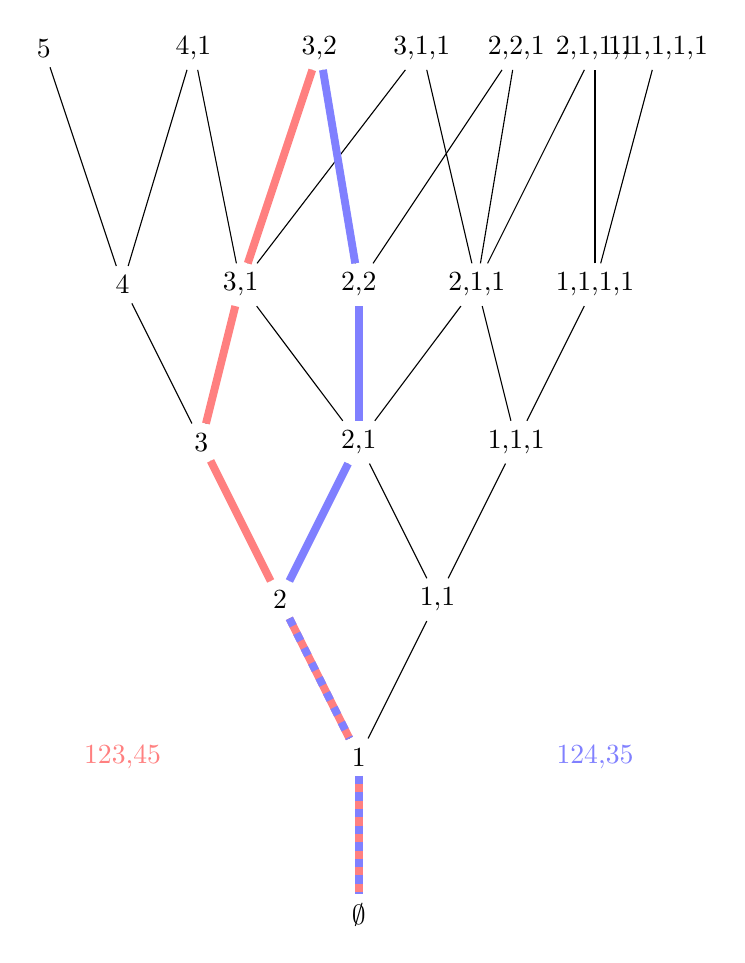
\begin{tikzpicture}[yscale=2]
        \node (A) {\(\emptyset\)};
        \node (B) at (0, 1) {\ydiagram{1}};
        \node (C1) at (-1, 2) {\ydiagram{2}};
        \node (C2) at (1, 2) {\ydiagram{1,1}};
        \node (D1) at (-2, 3) {\ydiagram{3}};
        \node (D2) at (0, 3) {\ydiagram{2,1}};
        \node (D3) at (2, 3)  {\ydiagram{1,1,1}};
        \node (E1) at (-3, 4) {\ydiagram{4}};
        \node (E2) at (-1.5, 4) {\ydiagram{3,1}};
        \node (E3) at (0, 4) {\ydiagram{2,2}};
        \node (E4) at (1.5, 4) {\ydiagram{2,1,1}};
        \node (E5) at (3, 4) {\ydiagram{1,1,1,1}};
        \node (F1) at (-4, 5.5) {\ydiagram{5}};
        \node (F2) at (-2.1, 5.5) {\ydiagram{4,1}};
        \node (F3) at (-0.5, 5.5) {\ydiagram{3,2}};
        \node (F4) at (0.8, 5.5) {\ydiagram{3,1,1}};
        \node (F5) at (2, 5.5) {\ydiagram{2,2,1}};
        \node (F6) at (3, 5.5) {\ydiagram{2,1,1,1}};
        \node (F7) at (3.8, 5.5) {\ydiagram{1,1,1,1,1}};
        
        \draw (A) -- (B);
        \draw (B) -- (C1);
        \draw (B) -- (C2);
        \draw (C1) -- (D1);
        \draw (C1) -- (D2);
        \draw (C2) -- (D2);
        \draw (C2) -- (D3);
        \draw (D1) -- (E1);
        \draw (D1) -- (E2);
        \draw (D2) -- (E2);
        \draw (D2) -- (E3);
        \draw (D2) -- (E4);
        \draw (D3) -- (E4);
        \draw (D3) -- (E5);
        \draw (E1) -- (F1);
        \draw (E1) -- (F2);
        \draw (E2) -- (F2);
        \draw (E2) -- (F3);
        \draw (E2) -- (F4);
        \draw (E3) -- (F3);
        \draw (E3) -- (F5);
        \draw (E4) -- (F4);
        \draw (E4) -- (F5);
        \draw (E4) -- (F6);
        \draw (E5) -- (F6);
        \draw (E5) -- (F7);
        \draw [red!50, line width=1mm] (F3) -- (E2);
        \draw [red!50, line width=1mm] (E2) -- (D1);
        \draw [red!50, line width=1mm] (D1) -- (C1);
        \draw [red!50, line width=1mm] (C1) -- (B);
        \draw [red!50, line width=1mm] (B) -- (A);
        \draw [blue!50, line width=1mm] (F3) -- (E3);
        \draw [blue!50, line width=1mm] (E3) -- (D2);
        \draw [blue!50, line width=1mm] (D2) -- (C1);
        \draw [blue!50, line width=1mm, dashed] (C1) -- (B);
        \draw [blue!50, line width=1mm, dashed] (B) -- (A);
        \ytableausetup{boxsize=1.5em}
        \begin{scope}[color=red!50]
            \node at (-3, 1) {\ytableaushort{123,45}};
        \end{scope}
        \begin{scope}[color=blue!50]
            \node at (3, 1) {\ytableaushort{124,35}};
        \end{scope}
    \end{tikzpicture}
    \caption{Paths in a Young lattice and the corresponding standard tableaux.}
    \label{fig:young lattice paths}
\end{figure}

This shows that in the repeated-restriction process above we get all standard tableau of shape \(\lambda\) appearing in the decomposition of the \(S_n\)-module restricted to an \(S_0\)-module.
That is, we have as modules
\begin{equation}
    \Res^{S_n}_{S_0} V_\lambda = \bigoplus_{T \in \standardYoungTableaux(\lambda)} V_T
\end{equation}
where \(V_T\) are 1-dimensional vector spaces.
Note that as vector spaces \(\Res^{S_n}_{S_0} V_\lambda = V_\lambda\), which gives us the following result.

\begin{dfn}{Gelfand--Zetlin Basis}{}
    The process detailed above defines, up to normalisation, a basis of \(V_\lambda\), known as the \defineindex{Gelfand--Zetlin basis}.
    Specifically, we let \(V_T = \field v_T\) then \(\{v_T \mid T \in \standardYoungTableaux(\lambda)\}\) is a basis of \(V_\lambda\).
\end{dfn}

Suppose that \(\Char \field \nmid n!\), so that \(\field S_n\) is semisimple.
Then we have the decomposition
\begin{equation}
    \field S_n \isomorphic \bigoplus_{\lambda \partition n} \End(V_\lambda) \isomorphic \bigoplus_{\lambda \partition n} \Mat_{\dim V_\lambda}(\complex).
\end{equation}
We can thus specify a subalgebra of \(\field S_n\)

\begin{dfn}{Gelfand--Zetlin Subalgebra}{}
    The \defineindex{Gelfand--Zetlin subalgebra}, \(A_n \subseteq \field S_n\), is the subalgebra consisting of elements whose action is diagonal in all irreducible representations.
\end{dfn}

That is, the Gelfand--Zetlin subalgebra consists of all elements of \(\field S_n\) which correspond to a direct sum of diagonal matrices in the above decomposition.

\begin{lma}{}{}
    The Gelfand--Zetlin subalgebra is a maximal commutative subalgebra of \(\field S_n\).
    Further, the Gelfand--Zetlin subalgebra is semisimple.
\end{lma}

The Gelfand--Zetlin basis element, \(v_T\), corresponds to the one-dimensional irreducible \(A_n\)-module, \(V_T = \field v_T\).

\section{Jucys--Murphy Elements}
\begin{dfn}{Jucys--Murphy Elements}{}
    The \(j\)th \defineindex{Jucys--Murphy element} of \(\field S_n\) is
    \begin{equation}
        L_j \coloneq \sum_{i=1}^j \cycle{i,j}.
    \end{equation}
    Note that \(L_1 = 0\) is the empty sum.
\end{dfn}

Note that
\begin{equation}
    L_n = \cycle{1,n} + \cycle{2,n} + \dotsb + \cycle{n-1,n}
\end{equation}
commutes with all of \(\field S_{n-1}\), since elements of \(\field S_{n-1}\) fix \(n\) and so if \(w \in S_{n-1}\) then \(L_n w\) is just \(L_n\) with the order of the terms in the sum rearranged.

This means that the Jucys--Murphy elements generate a commutative subalgebra of \(\field S_n\).

\begin{lma}{}{}
    The Gelfand--Zetlin subalgebra, \(A_n\), is generated by either
    \begin{itemize}
        \item \(Z_0, \dotsc, Z_n \subseteq \field S_n\) for \(Z_i = Z(\field S_n)\); or
        \item \(L_1, \dotsc, L_n\).
    \end{itemize}
\end{lma}

\section{Young's Seminormal Form}
For \(\lambda\) a partition of \(n\) fix some vector \(v_{T_0} \in V_\lambda\) where \(T_0\) is the canonical tableau of shape \(\lambda\).
Let \(T\) be some standard tableau of shape \(\lambda\).
Define \(w_T \in S_n\) by \(T = w_T \action T_0\), where \(S_n\) acts on \(T\) by permuting the boxes according to their numbering.
Then we may define \(v_T = \pi_T(w_T \action v_{T_0}) \in V_\lambda = V_T\) where
\begin{equation}
    \pi_T \colon \bigoplus_{S \in \standardYoungTableaux(\lambda)} \twoheadrightarrow V_T
\end{equation}
is projection onto the corresponding term of the direct sum.

\begin{thm}{}{}
    The simple transpositions, \(s_i = \cycle{i,i+1}\), act on \(V_\lambda\) in such a way that
    \begin{equation}
        s_i \action v_T = 
        \begin{cases}
            v_{s_i \action T} & \text{if } s_i \action T \text{ is a standard tableau};\\
            0 & \text{else}.
        \end{cases}
    \end{equation}
    Define \(c_T(k) = j - i\) when \(T(i, j) = k\).
    Then
    \begin{equation}
        s_i \action v_T = \frac{1}{c_T(i + 1) - c_T(i)} v_T + \left( 1 + \frac{1}{c_T(i + 1) - c_T(i)} \right) v_{s_i \action T}
    \end{equation}
    and
    \begin{equation}
        L_j \action v_T = c_T(j) v_T.
    \end{equation}
\end{thm}

\chapter{Symmetric Functions}
\section{Kostka Numbers}
Recall that for a partition, \(\lambda \partition n\), the row group of \(\lambda\) is \(S_\lambda \isomorphic S_{\lambda_1} \times \dotsb \times S_{\lambda_\ell}\) where \(S_{\lambda_1}\) acts on \(\{1, \dotsc, \lambda_1\}\), \(S_{\lambda_2}\) acts on \(\{\lambda_1 + 1, \dotsc, \lambda_1 + \lambda_2\}\), and so on.
Consider the trivial representation of \(S_\lambda\), \(\complex\).
We can define an \(S_n\)-module by inducing this up:
\begin{equation}
    M_\lambda \coloneq \Ind^{S_n}_{S_\lambda} \complex.
\end{equation}

\begin{lma}{}{}
    With notation as above we have \(M_\lambda \isomorphic \complex S_n a_\lambda\).
\end{lma}

Recall that if \(e\) is an idempotent of the algebra \(A\) then
\begin{equation}
    \Hom_A(Ae, M) \isomorphic eM
\end{equation}
for any left \(A\)-module, \(M\).
We then have
\begin{equation}
    \Hom_{S_n}(M_\lambda, V_\mu) = \Hom_{S_n}(\complex S_n a_\lambda, V_\mu) \isomorphic a_\lambda V_\mu = a_\lambda \complex S_n b_\mu a_\mu.
\end{equation}
We also have that
\begin{equation}
    \dim(a_\lambda \complex S_n b_\mu a_\mu) = 
    \begin{cases}
        1 & \lambda = \mu,\\
        0 & \mu < \lambda.
    \end{cases}
\end{equation}

\begin{dfn}{Weight}{}
    Let \(\lambda\) be a partition of \(n\).
    Let \(\mu\) be a sequence of nonnegative integers, \(\mu = (\mu_1, \mu_2, \dotsc)\) such that \(\sum_i \mu_i = n\) (so a partition minus the requirement that the \(\mu_i\) be weakly decreasing).
    We call such a \(\mu\) a \defineindex{composition} of \(n\).
    We say that a semi-standard Young tableau of shape \(\lambda\) has weight \(\mu\) if \(i \in \{1, \dotsc, n\}\) appears in the labelling of boxes \(\mu_i\) times.
\end{dfn}

\begin{dfn}{Kostka Numbers}{}
    Let \(\lambda\) be a partition of \(n\) and \(\mu\) a composition of \(n\).
    The \define{Kostka numbers}\index{Kostka number}, \(K_{\lambda\mu}\), are the number of semistandard tableaux of shape \(\lambda\) and weight \(\mu\).
\end{dfn}

Writing \(\semistandardYoungTableaux(\lambda, \mu)\) for the set of semistandard Young tableaux of shape \(\lambda\) and weight \(\mu\) we have that
\begin{equation}
    K_{\lambda\mu} = \abs{\semistandardYoungTableaux}(\lambda, \mu).
\end{equation}

\begin{exm}{}{}
    Suppose \(\lambda = (3, 2)\) and \(\mu = (1, 1, 2, 1)\).
    Then \(K_{\lambda\mu}\) is the number of semistandard tableaux of shape \((3, 2)\) filled with one \(1\), one \(2\), two \(3\)s, and one \(3\).
    It's not hard to check that the only options are
    \ytableausetup{boxsize=1em}
    \begin{equation}
        \ytableaushort{123,34}\,,\quad \ytableaushort{124,33}\,,\qand \ytableaushort{133,24}\,.
    \end{equation}
    Thus, \(K_{(3,2)(1,1,2,1)} = 3\).
    
    Any partition, \(\lambda\), is also a composition.
    In general, we have \(K_{\lambda\lambda} = 1\), since the only way to fill a Young diagram of shape \(\lambda\) with \(\lambda_1\) \(1\)s, \(\lambda_2\) \(2\)s, and so on in such a way that the result is semistandard is to have the first row filled with \(1\)s, the second row filled with \(2\)s, and so on.
    
    If \(\mu = (1, 1, \dotsc, 1)\) with \(n\) \(1\)s then every number from \(1\) to \(n\) appears exactly once, and being semistandard is the same as being standard.
    Thus,
    \begin{equation}
        K_{\lambda(1, 1, \dotsc, 1)} = f^\lambda = \abs{\standardYoungTableaux(\lambda)} = \dim V_\lambda = \frac{n!}{\lambda \intterobang}.
    \end{equation}
\end{exm}

\begin{prp}{}{}
    With notation as above we have that
    \begin{equation}
        M_\lambda = V_\lambda \oplus \vphantom{\bigoplus}\smash{\bigoplus_{\mu > \lambda}} K_{\mu\lambda} V_\mu.
    \end{equation}
\end{prp}

\section{Frobenius Character Formula for \texorpdfstring{\(S_n\)}{Sn}}
Consider the ring of polynomials in \(n\)-commuting indeterminates, \(\complex[x_1, \dotsc, x_n]\).
There is a natural action of the symmetric group, \(S_n\), on this ring, specifically
\begin{equation}
    (w \action f)(x_1, \dotsc, x_n) = f(x_{w^{-1}(1)}, \dotsc, x_{w^{-1}(n)}).
\end{equation}
Note that the action is defined in terms of \(w^{-1}\) simply because this is what gives us a left action.

Some polynomials in \(\complex[x_1, \dotsc, x_n]\) are left invariant under this action.
That is, if we permute the variables the polynomial doesn't change.
The following are some examples of this in three variables:
\begin{equation}
    \label{eqn:example symmetric polynomials}
    xyz, \quad xy + xz + yz, \quad x + y + z, \quad x^2y + x^2z + y^2x + y^2z + z^2x + z^2y.
\end{equation}

\begin{ntn}{Fixed Points}{}
    Let \(X\) be a set with some specified action of a group, \(G\).
    Write \(X^G\) for the set of fixed points of \(X\) under this action.
    That is,
    \begin{equation}
        X^G = \{x \in X \mid g \action x = x \forall g \in G\}.
    \end{equation}
\end{ntn}

We will now study \(\Lambda_n \coloneq \complex[x_1, \dotsc, x_n]^{S_n}\), and the generalisation of this to infinitely many variables.
We call elements of \(\Lambda_n\) \define{symmetric polynomials}\index{symmetric polynomial} in \(n\) variables.
First, notice that the product of two such polynomials is once again symmetric, as is their sum.
Thus, \(\Lambda_n\) is a ring.
Further, if any complex multiple of a symmetric function is again symmetric, and thus \(\Lambda_n\) is a \(\complex\)-algebra.

\begin{dfn}{Power Sums}{}
    Let \(r \in \integers_{\ge 0}\), and define the \defineindex{power sum}, \(p_r \in \complex[x_1, \dotsc, x_n]\) by
    \begin{equation}
        p_r(x_1, \dotsc, x_n) \coloneq \sum_{i=1}^n x_i^r.
    \end{equation}
\end{dfn}

First note that \(p_r\) is a symmetric polynomial.
Permuting the variables just rearranges the order of the \(x_i^r\) in the sum, which doesn't change the polynomial.

It turns out that the power sums generate all of \(\Lambda_n\).

\begin{prp}{}{}
    We have
    \begin{equation}
        \complex[x_1, \dotsc, x_n]^{S_n} \isomorphic \complex[p_1, \dotsc, p_n].
    \end{equation}
\end{prp}

Note that we are not considering \(\complex[p_1, \dotsc, p_n]\) to be a polynomial ring.
Instead it is simply all polynomials in the \(p_r\) subject to the relations that follow from the definition of the \(p_r\) in terms of the \(x_i\).

Consider the examples of \cref{eqn:example symmetric polynomials}.
These are \(p_3\), \(p_2\), \(p_1\), and \(p_2p_1 - p_3\) respectively.

\begin{ntn}{}{}
    Let \(\lambda\) be a partition of \(n\), and suppose \(N \ge \ell(\lambda)\) (which you'll recall is the number of nonzero terms in \(\lambda\)).
    Then we write
    \begin{equation}
        x^\lambda = x_1^{\lambda_1} x_2^{\lambda_2} \dotsm x_N^{\lambda_N}.
    \end{equation}
    Note that \(\lambda_i\) may be zero for some of these exponents.
    We also write
    \begin{equation}
        p_{\lambda} = p_{\lambda_1} p_{\lambda_2} \dotsm p_{\lambda_{\ell(\lambda)}}.
    \end{equation}
    Note that this is the same as if we carry on all the way to \(x_N\), since \(p_0 = 1\).
    
    We also define the sum of partitions in the obvious way, so \((\lambda + \rho)_i = \lambda_i + \rho_i\).
    
    The antisymmetric polynomial
    \begin{equation}
        \Delta(x) = \prod_{1 \le i < j \le N} (x_i - x_j)
    \end{equation} 
    is called the \defineindex{van der Monde determinant}.
\end{ntn}

\begin{prp}{}{}
    Let \(\lambda\) be a partition of \(n\).
    For \(N \ge \ell(\lambda)\) we have the following relationship between characters and symmetric polynomials in \(N\) variables:
    \begin{itemize}
        \item \(\chi_{M_\lambda}(\mu)\) is the coefficient of \(x^\lambda\) in \(p_\mu\); and
        \item \(\chi_{V_\lambda}(\mu)\) is the coefficient of \(x^{\lambda + \rho}\) in \(\Delta(x)p_\mu\).
    \end{itemize}
    Note that \(\chi_{X}(\mu)\) means the character of any element of the conjugacy class labelled by cycle-type \(\mu\) in the representation \(X\).
\end{prp}

\section{The Ring of Symmetric Functions}
The previous result suggests that there is a close relationship between the representation theory of \(S_n\) and symmetric polynomials.
One thing that gets in the way when we try to utilise this connection is that we always have to have \enquote{enough} variables.
In the previous result this meant we had \(N \ge \ell(\lambda)\).
However, most things we can say about symmetric functions are fairly independent of the number of variables.
The way we get around this is to consider an infinite number of variables.
This takes a bit of care to set up properly, but then we can go back to thinking of the resulting elements as being symmetric polynomials in sufficiently many variables after we've put in the work upfront.

\subsection{Construction}
For this section we work with polynomials over \(\integers\).
This can then be extended to \(\complex\) by extension of scalars later.

Notice that
\begin{equation}
    \Lambda_N = \integers[x_1, \dotsc, x_N]^{S_N}
\end{equation}
is a graded ring, specifically,
\begin{equation}
    \Lambda_N = \bigoplus_{d \ge 0} \Lambda_N^d
\end{equation}
where \(\Lambda_N^d\) is the \(\integers\)-submodule of \(\Lambda_N\) consisting of homogeneous symmetric polynomials of degree \(d\).

Let \(\lambda = (\lambda_1 \ge \dotsb \ge \lambda_N \ge 0)\) be a partition of length at most \(N\) with \(\abs{\lambda} = d\).
We define the \defineindex{monomial symmetric polynomial} corresponding to \(\lambda\) to be
\begin{equation}
    m_\lambda(x_1, \dotsc, x_N) = \sum_{\alpha} x^\alpha
\end{equation}
where the sum is over all \(\alpha\) which are given by permuting the first \(N\) terms of \(\lambda\).
For example, if \(\lambda = (3,2)\) and \(N = 3\) then the permutations of the first three terms of \(\lambda\) are
\begin{equation}
    (3, 2, 0), \quad (3, 0, 2),\quad (2, 3, 0), \quad (2, 0, 3), \quad (0, 3, 2), \qand (0, 2, 3).
\end{equation}
Thus, we have
\begin{align}
    &m_{(3,2)}(x_1, x_2, x_3)\\
    &= x_1^3 x_2^2 x_3^0 + x_1^3 x_2^0 x_3^2 + x_1^2 x_2^3 x_3^0 + x_1^2 x_2^0 x_3^3 + x_1^0 x_2^3 x_3^2 + x_1^0 x_2^2 x_3^3 \notag\\
    &= x_1^3 x_2^2 + x_1^3 x_3^2 + x_1^2 x_2^3 + x_1^2 x_3^3 + x_2^3 x_3^2 + x_2^2 x_3^3. \notag
\end{align}
Note that \(m_{(r)} = p_r\).
This definition makes sense so long as \(N \ge \ell(\lambda)\), so if we want to consider all degree \(d\) polynomials then we should take \(N \ge d\), which we'll assume from now on.
Under these considerations the \(m_\lambda\) form a basis for \(\Lambda_N^d\).

For \(N' \ge N\) there is a surjection
\begin{equation}
    \rho_{N',N}^d \colon \Lambda_{N'}^d \twoheadrightarrow \Lambda_N^d
\end{equation}
defined by setting \(x_{N+1} = \dotsb = x_{N'} = 0\).
The action of this map on the monomial symmetric polynomials is
\begin{equation}
    \rho_{N',N}^d(m_\lambda(x_1, \dotsc, x_{N'})) = 
    \begin{cases}
        m_\lambda(x_1, \dotsc, x_N) & \ell(\lambda) \le N;\\
        0 & \text{otherwise}.
    \end{cases}
\end{equation}
Further, note that the map \(\rho_{N',N}^d\) is bijective for \(N' \ge N \ge d\).

We then have a sequence of bijections
\begin{equation}
    \Lambda_1^d \twoheadleftarrow \Lambda_2^d \twoheadrightarrow \Lambda_3^d \twoheadrightarrow \dotsb.
\end{equation}
This is an inverse system, by which we mean that \(\rho^d_{i,k} = \rho^d_{i,j} \circ \rho^d_{j,k}\) for all \(i, j, k \in \integers_{>0}\).
Define the ring of homogeneous functions of degree \(d\) to be the inverse limit
\begin{equation}
    \Lambda^d = \varprojlim_N \Lambda_N^d.
\end{equation}
That is, elements of \(\Lambda^d\) are sequences, \((f_N)_{N \in \integers_{> 0}}\), where each \(f_N\) is a homogeneous degree \(d\) polynomial in \(N\) variables.
These sequences are (by definition of the inverse limit) such that
\begin{equation}
    f_{N+1}(x_1, \dotsc, x_N, 0) = f_N(x_1, \dotsc, x_N).
\end{equation}

The projections, sending such a sequence to its \(N\)th term,
\begin{align}
    \proj^d_N \colon \Lambda^d &\twoheadrightarrow \Lambda^d_N,\\
    f = (f_N)_{N \in \integers_{>0}} &\mapsto f_N,
\end{align}
are isomorphisms for \(N \ge d\).
This means that \(\Lambda^d\) is a free \(\integers\)-module with basis \(\{m_\lambda \mid \lambda \partition d\}\).

We define the \defineindex{ring of symmetric functions} to be the graded ring
\begin{equation}
    \Lambda = \bigoplus_{d \ge 0} \Lambda^d.
\end{equation}

\begin{remark}{}{}
    Note that \emph{technically} elements of \(\Lambda\) are not polynomials, they are infinite sequences of polynomials.
    However, we can pretty much treat them as polynomials most of the time, just take some polynomial sufficiently far along in the sequence that there are enough variables to do whatever it is we're trying to do.
    To make this distinction we call elements of \(\Lambda\) \enquote{symmetric functions} instead of \enquote{symmetric polynomials}, but we pretty much think of them as polynomials.
    
    Let \(f_N\) and \(f_{N+1}\) be symmetric polynomials in \(N\) and \(N + 1\) variables respectively such that
    \begin{equation}
        f_N(x_1, \dotsc, x_N) = f_{N+1}(x_1, \dotsc, x_N, 0).
    \end{equation}
    If it's possible to make definitions of a family of polynomials in this way such that at each step adding a new variable and setting it to zero doesn't change anything then it makes sense to consider \((f_N)_{N \in \integers_{>0}}\) as an element of \(\Lambda\).
    We call this the projective limit of \(f\) (where \(f\) is some label referring to this whole family of polynomials, which we really want to think of as all being the same symmetric function).
\end{remark}

\begin{remark}{}{}
    There are several constructions of \(\Lambda\).
    The one we've given makes it an inverse limit in the category of graded rings.
    There is an alternative construction which makes it a direct limit in the category of rings of the direct system
    \begin{equation}
        \Lambda_1^d \hookrightarrow \Lambda_2^d \hookrightarrow \Lambda_3^d \hookrightarrow
    \end{equation}
    where the inclusions are defined in terms of another basis of polynomials, called the elementary symmetric polynomials, \(e_r\), and the maps defined by \(e_r(x_1, \dotsc, x_n) \mapsto e_r(x_1, \dotsc, x_n, x_{n+1})\).
    
    As categorical duals an inverse limit is some subset of the product, and the direct limit is some the disjoint union modulo some equivalence relation.
    There are benefits to both constructions.
    Elements of inverse limits are slightly easier to work with, because we don't have to keep track of the equivalence relation and worry if things are well-defined.
    Conversely, with the direct limit definition we can directly (no pun intended) identify (equivalence classes) of elements with elements of some object in the direct system.
    
    Once we place a grading on the ring of symmetric functions as defined in terms of a direct limit it is isomorphic to the ring of symmetric functions as defined in terms of an inverse limit.
    
    Since we won't have much reason to worry about the exact structure of elements of this ring we won't worry any more about exactly how it's defined.
\end{remark}

Let \(\Lambda\) be the ring of symmetric functions with integer coefficients.
Then for any ring, \(R\), we can define \(\Lambda_R = \Lambda \otimes_{\integers} R\), to be the ring of symmetric functions with coefficients in \(R\).
In particular, \(\Lambda_{\complex}\) is the ring of symmetric functions with coefficients in \(\complex\).

\begin{prp}{}{}
    We have that
    \begin{equation}
        \Lambda_{\complex} \isomorphic \complex[p_1, p_2, \dotsc]
    \end{equation}
    where the \(p_r\) are the projective limits of the power sums.
\end{prp}

\section{Schur Functions}
\begin{dfn}{Schur Polynomial}{}
    Let \(\lambda\) be a partition of length \(N\).
    We define the corresponding \define{Schur polynomial}\index{Schur!polynomial} to be
    \begin{equation}
        s_\lambda(x) \coloneq \frac{\det(x_i^{\lambda_j + N - j})_{1 \le i, j \le N}}{\det(x_i^{N-j})_{1\le i,j\le N}}.
    \end{equation}
\end{dfn}

Schur polynomials are stable, in the sense that if \(s_\lambda\) is the Schur polynomial in \(N\) variables, and \(\hat{s}_\lambda\) is the Schur polynomial in \(N + 1\) variables then
\begin{equation}
    s_\lambda(x_1, \dotsc, x_N) = \hat{s}_\lambda(x_1, \dotsc, x_N, 0).
\end{equation}
In practice both of these are denoted \(s_\lambda\) with the number of variables distinguishing them.
Since \(s_\lambda\) is unchanged by adding more variables the setting them to zero we can consider the projective limit of the Schur polynomials.

\begin{dfn}{Schur Function}{}
    Let \(\lambda\) be a partition.
    The corresponding \defineindex{Schur function} is the projective limit of the Schur polynomials \(s_\lambda\) as we increase the number of variables.
\end{dfn}

\begin{thm}{}{}
    The Schur functions form a \(\integers\)-basis, \(\{s_\lambda \mid \lambda \partition n, n \in \integers_{\ge 0}\}\), of \(\Lambda\).
\end{thm}

By a \(\integers\)-basis we mean that any symmetric function with integer coefficients can be expressed as a linear combination of Schur functions with integer coefficients.
In other words, the \(s_\lambda\) form a basis of \(\Lambda = \Lambda_{\integers}\).
This is in contrast to the \(p_\lambda\) which form only a \(\rationals\)-basis of \(\Lambda_{\rationals}\).

With these constructions we can restate the Frobenius formula as
\begin{equation}
    p_\mu = \sum_\lambda \chi_{V_\lambda}(\mu) s_\lambda.
\end{equation}

\section{Macdonald's Characteristic Map}
For \(w \in S_n\) we denote by \(\mu(w) = (\mu_1 \ge \mu_2 \ge \dotsb \ge \mu_n \ge 0)\) the ordered cycle length of \(w\).
So, for example, in \(S_5\) if \(w = \cycle{1,2,3}\cycle{4,5}\) then \(\mu(w) = (3, 2)\).
We can then define a map
\begin{align}
    \psi \colon S_n &\to \Lambda\\
    w &\mapsto p_{\mu(w)} = p_{\mu_1} \dotsm p_{\mu_n}.
\end{align}
Since this map is defined only by the cycle type of \(w\) we have that \(\psi(w) = \psi(w')\) whenever \(w\) and \(w'\) are conjugate.

We have the obvious embedding \(S_m \times S_n \hookrightarrow S_{m + n}\), in which \(w \times w' \mapsto u\) defined by
\begin{equation}
    u(i) =
    \begin{cases}
        w(i) & i \in \{1, \dotsc, m\};\\
        w'(i) & i \in \{m + 1, \dotsc, m + n\}.
    \end{cases}
\end{equation}
Then we have
\begin{equation}
    \psi(w \times w') = \psi(w) \psi(w').
\end{equation}
Recall that \(\classFunctions_n = \classFunctions_n(S_n)\) is the space of class functions, \(S_n \to \complex\), and that this is spanned by the irreducible characters \(\{\chi_\lambda \mid \lambda \partition n\}\).

We may then consider the (vector space) direct sum
\begin{equation}
    \classFunctions = \bigoplus_{n \ge 0} \classFunctions_n
\end{equation}
where \(\classFunctions_0 = \complex\).
This graded vector space can be made into a graded ring by defining multiplication of homogeneous basis elements:
\begin{equation}
    \chi_\lambda * \chi_\mu \coloneq (\chi_\lambda \times \chi_\mu) \uparrow^{S_{m+n}}_{S_m \times S_n}.
\end{equation}
In words, we define the product of irreducible characters to be the induced character of the representation arising from the obvious embedding \(S_m \times S_n \hookrightarrow S_{m + n}\).

Any \(f, g \in \classFunctions\) may be expanded as a sum of \(f_n, g_n \in \classFunctions_n\):
\begin{equation}
    f = \sum_{n \ge 0} f_n, \qand g = \sum_{n \ge 0} g_n.
\end{equation}
Recall that we've defined an inner product, \(\innerprod{-}{-}_{S_n} \colon \classFunctions_n \times \classFunctions_n \to \complex\).
We can extend this to an inner product, \(\innerprod{-}{-} \colon \classFunctions \times \classFunctions \to \complex\), by defining
\begin{equation}
    \innerprod{f}{g} = \sum_n \innerprod{f_n}{g_n}_{S_n}.
\end{equation}
This is the obvious extension given by declaring that the different homogeneous subspaces are orthogonal.

\begin{dfn}{Macdonald's Characteristic Map}{}
    \defineindex{Macdonald's characteristic map} is the map \(\ch \colon \classFunctions \to \Lambda_{\complex}\) defined on homogenous \(f \in \classFunctions_n\) by
    \begin{equation}
        \ch(f) = \innerprod{f}{\psi}_{S_n} = \frac{1}{n!} \sum_{w \in S_n} f(w)\psi(w).
    \end{equation}
\end{dfn}

\begin{lma}{}{}
    With the notation as above
    \begin{equation}
        \ch(f) = \sum_{\lambda \partition n} \frac{f_\mu}{z_\mu} p_\mu
    \end{equation}
    where \(f_\mu\) is the value of \(f\) on any element of the conjugacy class of cycle type \(\mu\), and \(z_\mu\) is the size of the conjugacy class of cycle type \(\mu\).
\end{lma}

\begin{dfn}{Hall Inner Product}{}
    The \defineindex{Hall inner product} on \(\Lambda\) is defined by
    \begin{equation}
        \innerprod{p_\lambda}{p_\mu} = \delta_{\lambda\mu} z_\mu
    \end{equation}
    with \(z_\mu\) the size of the conjugacy class of cycle type \(\mu\).
\end{dfn}

\begin{thm}{}{}
    The ring \(\classFunctions\) is isomorphic to \(\Lambda\) with the isomorphism given by \(\ch(\chi_\lambda) = s_\lambda\).
    Further, this is an isometry with respect to the two inner products we've just defined.
    That is, \(\innerprod{\ch(f)}{\ch(g)} = \innerprod{f}{g}_{S_n}\) for homogeneous \(f, g \in \classFunctions_n\).
    \begin{proof}
        To show that this is a ring homomorphism we have the following
        \begin{align}
            \ch(f * g) &= \innerprod{\Ind^{S_{m+n}}_{S_m \times S_n} f \otimes g}{\psi}_{S_{m+n}}\\
            &= \innerprod{f \otimes g}{\Res^{S_{m+n}}_{S_m \times S_n} \psi}_{S_{m\times n}}\\
            &= \innerprod{f}{\psi}_{S_m} \innerprod{g}{\psi}_{S_n}\\
            &= \ch(f) \ch(g).
        \end{align}
        The Hall inner product is defined exactly such that this map is an isometry.
        Finally, since the \(\chi_\lambda\) are a basis of \(\classFunctions_n\) and the \(s_\lambda\) are a basis of \(\Lambda^n\) for \(\lambda \partition n\) then \(\ch\) is an isomorphism.
    \end{proof}
\end{thm}

\begin{thm}{}{}
    Consider the following maps:
    \begin{itemize}
        \item \(\ch \colon \classFunctions \to \Lambda_{\complex}\);
        \item \(\classFunctions \to Z = \bigoplus_{n \ge 0} Z(\complex S_n)\) given by \(\chi_\lambda \mapsto c_\lambda\);
        \item the Frobenius map \(F \colon Z \to \Lambda_{\complex}\) given by \(F(c_\lambda) = p_\mu/z_\mu\).
    \end{itemize}
    These are isomorphisms, and the following diagram of these algebra isomorphisms commutes:
    \begin{equation}
        \begin{tikzcd}
            \classFunctions \arrow[r] \arrow[dr] & Z \arrow[d]\\
            & \Lambda_{\complex}\mathrlap{.}
        \end{tikzcd}
    \end{equation}
\end{thm}

\begin{crl}{}{}
    If \(\lambda\) is a partition of \(n\) then
    \begin{equation}
        s_\lambda = \sum_{\mu \partition n} \frac{\chi_\lambda(\mu)}{z_\mu} p_\mu.
    \end{equation}
\end{crl}

\begin{remark}{}{}
    The above diagram can be further extended via the boson--fermion correspondence to
    \begin{equation}
        \begin{tikzcd}
            \classFunctions \arrow[r] \arrow[dr] \arrow[d] & Z \arrow[d]\\
            \bigwedge^{\infty/2} V \arrow[r] & \Lambda_{\complex}
        \end{tikzcd}
    \end{equation}
    where \(V = \bigoplus_{n \in \integers} \complex v_n\) and \(\bigwedge^{\infty/2}V\) is defined to consist of all semi-infinite wedge products of the form
    \begin{equation}
        v_{i_1} \wedge v_{i_2} \wedge v_{i_3} \wedge \dotsb.
    \end{equation}
    The isomorphism \(\bigwedge^{\infty/2}V \isomorphic \Lambda_{\complex}\) is called the boson-fermion correspondence.
    The details of this map are beyond the scope of this remark.
\end{remark}

\section{More Symmetric Functions}
We have already seen three families of symmetric functions, \(p_\lambda\), \(m_\lambda\), and \(s_\lambda\).
Of these we've seen that \(s_\lambda\) are the images of irreducible characters under Macdonald's characteristic map.
The \(m_\lambda\) are the images of the characters \(\chi_{M_\lambda}\) under Macdonald's characteristic map.
A corollary of this is that
\begin{equation}
    m_\lambda = \sum_{\mu \partition n} K_{\mu\lambda} s_\mu.
\end{equation}
Note that this means that the expansion of \(m_\lambda\) in terms of Schur functions has only nonnegative coefficients, a property known as \define{Schur positivity}\index{Schur!positivity}.

Characters of other representations likewise give us families of symmetric polynomials.
In particular the \define{complete symmetric functions}\index{complete symmetric function},
\begin{equation}
    h_n = \sum_{i_1 \le \dotsb \le i_n} x_{i_1} \dotsm x_{i_n},
\end{equation}
are the images of the trivial character, \(\chi_{(n)}\), under this map.
Note that this means that \(h_n = s_{(n)}\).
Similarly, the \define{elementary symmetric functions}\index{elementary symmetric function},
\begin{equation}
    e_n = \sum_{i_1 < \dotsb < i_n} x_{i_1} \dotsm x_{i_n},
\end{equation}
are the images of the sign character, \(\chi_{(1, \dotsc, 1)}\), under the Macdonald characteristic map.
Note that this means that \(e_n = s_{(1, \dotsc, 1)}\).

We can use various relationships in the representation theory of the symmetric group to derive results about the symmetric polynomials.
For example, the decomposition of \(M_\lambda\) as
\begin{equation}
    V_\lambda \oplus \vphantom{\bigoplus}\smash{\bigoplus_{\mu > \lambda}} K_{\mu\lambda} V_\mu
\end{equation}
factors through Macdonald's characteristic map to tell us that
\begin{equation}
    h_\lambda = s_\lambda + \sum_{\mu > \lambda} K_{\mu\lambda}s_\mu.
\end{equation}
Recalling that \(M_\lambda\) is defined by inducing the trivial representation of the row group, \(S_\lambda\), we can also induce the sign representation of \(S_\lambda\) to get a similar decomposition which gives us
\begin{equation}
    e_{\lambda'} = s_{\lambda} + \sum_{\mu < \lambda} K_{\mu' \lambda'} s_\mu.
\end{equation}

The \define{Pieri rules}\index{Pieri rule} arise when we consider what happens if we induce the representation \(\complex \otimes V_\lambda\) or \(\complex_{-} \otimes V_\lambda\) (where \(\complex_{-}\) is the sign representation) of \(S_m \times S_n\) up to \(S_{m+n}\).
The first gives
\begin{equation}
    h_m s_\mu = \sum_{\substack{\lambda \partition n\\ \lambda \setminus \mu \text{ horiz. strip}}} s_\lambda
\end{equation}
and the second gives
\begin{equation}
    e_m s_\mu =  \sum_{\substack{\lambda \partition n\\ \lambda \setminus \mu \text{ vert. strip}}} s_\lambda.
\end{equation}
Note that \(\lambda \setminus \mu\) is a \defineindex{horizontal strip} if it has at most one box in each column, and a \defineindex{vertical strip} if it has at most one box in each row.

\section{Littlewood--Richardson Rule}
\begin{dfn}{Littlewood--Richardson Coefficient}{}
    Given a tableau we can form a word by concatenating the reversed rows from top to bottom.
    We say that the result of doing this is a \defineindex{lattice word} if any prefix has at least as many \(1\)s as it does \(2\)s, at least as many \(2\)s as it does \(3\)s and so on.
    When the word of a tableau is a lattice word we call it a \define{Littlewood--Richardson tableau}\index{Littlewood--Richardson!tableau}.
    
    The \define{Littlewood--Richardson coefficient}\index{Littlewood--Richardson!coefficient}, \(c_{\lambda\mu}^\nu\), is defined to be the number of of shape \(\nu \setminus \lambda\) and weight \(\mu\).
\end{dfn}

\begin{thm}{Littlewood--Richardson Rule}{}
    \index{Littlewood--Richardson!rule}
    Let \(\lambda\) and \(\mu\) be partitions.
    Then
    \begin{equation}
        s_\lambda s_\mu = \sum_{\nu} c^\nu_{\lambda\mu} s_\nu.
    \end{equation}
\end{thm}

The Littlewood--Richardson rule is a famously tricky result to prove, requiring some careful combinatorics.
There are several related statements to the rule above.

One result which follows immediately is that if we have the simple \(S_{\abs{\lambda}}\) and \(S_{\abs{\mu}}\) modules \(V_\lambda\) and \(V_\mu\) then we that, as \(S_{\abs{\nu}}\)-modules, where \(\abs{\nu} = \abs{\lambda} + \abs{\mu}\), we have
\begin{equation}
    \Ind^{S_{\abs{\nu}}}_{S_{\abs{\lambda}} \times S_{\abs{\mu}}} (V_\lambda \otimes V_\mu) = \bigoplus_{\nu} c^\nu_{\lambda\mu} V_\nu
\end{equation}
as \(S_{m + n}\)-modules.
Conversely, we also have
\begin{equation}
    \Res^{S_{\abs{\nu}}}_{S_{\abs{\lambda} \times S_{\abs{\mu}}}} V_\nu = \bigoplus_{\lambda,\mu} c^\nu_{\lambda\mu} V_\lambda \otimes V_\mu
\end{equation}
as \((S_m \times S_n)\)-modules.

Another result, which is related to this one via Schur--Weyl duality, is that simple \(\specialLinear_n(\complex)\)-modules can be labelled by partitions, call such a module \(E_\lambda\), and then we have
\begin{equation}
    E_\lambda \otimes E_\mu = \bigoplus_{\nu} c^\nu_{\lambda\mu}E_\nu.
\end{equation}

In fact, it turns out that the Schur functions can be realised as the characters of these irreducible representations, and as such this is really a more general version of the Littlewood--Richardson rule as stated above, it's a sort of categorification of the rule.

\section{Application: Intersection Cohomology of Grassmannians}
Recall that the Grassmannian, \(\Gr_k(\complex^n)\), is defined to be the set of \(k\)-dimensional subspaces of \(\complex^n\).
An element of \(\Gr_k(\complex^n)\) can be represented as a \(k \times n\) matrix, specifically, it's the row space of this matrix.
This doesn't give a unique representation of our subspace, but we can fix a unique representation by placing the matrix into reduced row echelon form, which doesn't change the row space.
There are then \(k\) columns which are \(0\) apart from a single \(1\) (the pivot).
The entries in the other \(n - k\) columns determine exactly which \(k\)-dimensional subspace we're considering.
These \(k(n-k)\) entries can then be interpreted as coordinates, which makes \(\Gr_k(\complex^n)\) into a \(k(n - k)\)-dimensional complex manifold.

For example, consider \(\Gr_4(\complex^8)\), one particular subspace of this has pivots in columns \(2\), \(3\), \(5\), and \(8\), so it looks like
\begin{equation}
    \begin{pmatrix}
        * & 1 & 0 & * & 0 & * & * & 0\\
        * & 0 & 1 & * & 0 & * & * & 0\\
        * & 0 & 0 & * & 1 & * & * & 0\\
        * & 0 & 0 & * & 0 & * & * & 1
    \end{pmatrix}
    .
\end{equation}
The \(*\)s represent values that we are free to vary.
The above is the standard reduced row echelon form, but it will be more useful for us to use a slightly different convention, in which the left-most pivot appears lowest, so we would instead have
\begin{equation}
    \begin{pmatrix}
        * & 0 & 0 & * & 0 & * & * & 1\\
        * & 0 & 0 & * & 0 & * & * & 0\\
        * & 0 & 1 & * & 0 & * & * & 0\\
        * & 1 & 0 & * & 0 & * & * & 0
    \end{pmatrix}
    .
\end{equation}

We can turn such a matrix into a Young diagram as follows.
Take \(i_1\) to be the left-most nonzero column, \(i_2\) to be the left-most nonzero column linearly independent from \(i_1\), and so on.
Then we can use row operations to write the matrix so that there are pivots in columns \(i_j\), each column before \(i_1\) is just \(0\) (this is already the case) and each column between \(i_j\) and \(i_{j+1}\) starts with \(k - j\) zeros.
For example, with the (second) matrix form above, where the pivots appear in rows \(2\), \(3\), \(5\), and \(8\) we can basically set the first \(k - j\) \(*\)s to be \(0\) up to column \(i_j\):
\begin{equation}
    \begin{pmatrix}
        0 & 0 & 0 & 0 & 0 & 0 & 0 & 1\\
        0 & 0 & 0 & 0 & 0 & * & * & 0\\
        0 & 0 & 1 & * & 0 & * & * & 0\\
        0 & 1 & 0 & * & 0 & * & * & 0
    \end{pmatrix}
    .
\end{equation}
Finally, delete the rows with the pivots, and we are left with
\begin{equation}
    \begin{pmatrix}
        0 & 0 & 0 & 0\\
        0 & 0 & * & *\\
        0 & * & * & *\\
        0 & * & * & *
    \end{pmatrix}
    .
\end{equation}
Interpreting the \(0\)s as boxes in our Young diagram gives
\begin{equation}
    \ydiagram{4,2,1,1}\,.
\end{equation}

Conversely, given a partition, \(\lambda\), we can consider the subset, \(\Omega_\lambda^{\circ} \subseteq \Gr_k(\complex^n)\), of all subspaces of \(\complex^n\) which have \(\lambda\) as their corresponding Young diagram.
We call this a Schubert cell.
We call the closure, \(\Omega_\lambda\), of one of these cells a Schubert variety.

It turns out that the cohomology of \(\Gr_k(\complex^n)\) is a freely generated abelian group on the classes \(\sigma_\lambda = [\Omega_\lambda]\) as \(\lambda\) ranges over all Young diagrams with at most \(k\) rows and \(n - k\) columns.
This is a general fact about the cohomology of spaces admitting such a cellular decomposition.

Given a space, \(X\), with a cohomology theory we can define the cohomology ring to be
\begin{equation}
    H^{\bullet}(X) = \bigoplus_m H^m(X).
\end{equation}
The product in this ring is given by the cup product, the details of which are beyond the scope of this course.
However, in this case the product turns out to be given by
\begin{equation}
    \sigma_\lambda \sigma_\mu = \sum_\nu c^{\nu}_{\lambda\mu} \sigma_\nu.
\end{equation}
It turns out that the cohomology ring, \(H^*(\Gr(k; \complex^n))\), has the presentation
\begin{equation}
    H^{\bullet}(\Gr(k; \complex^n)) \isomorphic \Lambda / I_{k,n}
\end{equation}
where \(I_{k,n}\) is the ideal generated by Schur functions \(s_\lambda\) where the Young diagram of \(\lambda\) has more than \(k\) rows or more than \(n - k\) columns, so it doesn't fit in a \(k \times (n - k)\) bounding box.
The isomorphism is given by mapping a Schubert class to a Schur function, \(\sigma_\lambda \mapsto s_\lambda\).
Thus, the multiplication in the cohomology ring is nothing but the multiplication of Schur functions indexed by partitions fitting into a \(k \times (n - k)\) bounding box.
In this context the Littlewood--Richardson coefficients have an interpretation as the intersection numbers.

\section{Hopf Algebra Structure}
\textit{For more details on Hopf algebras see my notes from the Hopf algebras course (\url{https://github.com/WilloughbySeago/phd-courses-notes/tree/main/hopf-algebras}).}

The ring of symmetric functions with coefficients in \(\complex\), \(\Lambda = \Lambda_{\complex}\), is a commutative and cocommutative Hopf algebra.
First, note that we can identify \(\Lambda \otimes \Lambda\) with \(\Lambda\).
The comultiplication is given by
\begin{equation}
    \Delta(s_\lambda) = \sum_{\mu} s_{\lambda\setminus \mu} \otimes s_\mu
\end{equation}
where \(s_{\lambda \setminus \mu}\) is the skew Schur function defined by
\begin{equation}
    s_{\lambda \setminus \mu} = \sum_\nu c^\lambda_{\mu\nu} s_\nu.
\end{equation}
Thus,
\begin{equation}
    \Delta(s_\lambda) = \sum_{\mu, \nu} c^\lambda_{\mu\nu} s_{\nu} \otimes s_\mu.
\end{equation}
Note that this is cocommutative since \(c^\lambda_{\mu\nu}\) is symmetric in \(\mu\) and \(\nu\).
In terms of power sums this comultiplication is given by
\begin{equation}
    \Delta(p_r) = p_r \otimes 1 + 1 \otimes p_r.
\end{equation}
The comultiplication on an arbitrary symmetric function, \(f\), is
\begin{equation}
    \Delta(f) = \sum_\mu s_\mu^{\perp} f \otimes s_\mu
\end{equation}
where \(s_\mu^{\perp}\) is the adjoint of \(s_\mu\) with respect to the Hall inner product.

The counit is given by \(\varepsilon(1) = 1\) and \(\varepsilon(f) = 0\) for all homogeneous symmetric functions, \(f\), of degree greater than zero.
In other words, \(\varepsilon(f)\) (for \(f\) not necessarily homogeneous) is simply the constant term of \(f\).

The antipode is given by
\begin{equation}
    \chi(s_\lambda) = (-1)^{\abs{\lambda}} s_{\lambda'}.
\end{equation}

The ring \(\Lambda \otimes \Lambda\) inherits the inner product of \(\Lambda\), namely
\begin{equation}
    \innerprod{f \otimes g}{f' \otimes g'}_{\Lambda \otimes \Lambda} = \innerprod{f}{f'}_{\Lambda} \innerprod{g}{g'}_{\Lambda}.
\end{equation}
The ring \(\classFunctions\), which we've shown to be isomorphic to \(\Lambda\), inherits the Hopf algebra structure of \(\Lambda\).
Then, if we take class functions, \(\varphi, \gamma, \eta \in \classFunctions\), such that \(f = \ch(\varphi)\), \(g = \ch(\gamma)\), and \(h = \ch(\eta)\) Frobenius reciprocity tells us that
\begin{equation}
    \innerprod{\Res^{S_{m+n}}_{S_m \times S_n} \varphi}{\gamma \otimes \eta}_{S_m \times S_n} = \innerprod{\varphi}{\Ind^{S_{m+n}}_{S_m \times S_n} (\gamma \otimes \eta)}_{S_{m + n}}.
\end{equation}
Going back to \(\Lambda\) this tells us that
\begin{equation}
    \innerprod{\Delta(f)}{g \otimes h}_{\Lambda \otimes \Lambda} = \innerprod{f}{gh}_{\Lambda}.
\end{equation}

From this fact it follows that the Hopf algebra structure of \(\Lambda\) is self-dual, and in particular that
\begin{equation}
    \innerprod{\Delta(s_\lambda)}{s_\mu \otimes s_\nu}_{\Lambda \otimes \Lambda} = \innerprod{s_\lambda}{s_\mu s_\nu} = c^\lambda_{\mu\nu},
\end{equation}
giving yet another interpretation of the Littlewood--Richardson coefficients.

\section{Another Product}
We induced a product structure on the class functions by defining a product on the symmetric functions.
We can go the other way around, and use the product on homogeneous class functions, \(\varphi\) and \(\psi\), to induce a product, \(\cdot\), on the corresponding symmetric functions.
Essentially, we require that \(\ch\) is a homomorphism with respect to this product, so
\begin{equation}
    \ch(\varphi) \cdot \ch(\psi) = \ch{\varphi \psi}
\end{equation}
for \(\varphi, \psi \in \classFunctions_n\).
Then, taking all partitions to be partitions of \(n\), we have
\begin{equation}
    s_\lambda \cdot s_\mu = \sum_\nu \gamma^\nu_{\lambda\mu} s_\nu
\end{equation}
where
\begin{equation}
    \gamma^\nu_{\lambda\mu} = \innerprod{\chi_\nu}{\chi_\lambda \chi_\mu}_{S_n}.
\end{equation}
The power sums are unnormalised idempotents with respect to this product, that is
\begin{equation}
    p_\lambda \cdot p_\mu = \delta_{\lambda\mu} z_\mu p_\mu
\end{equation}
where \(z_\mu\) is the size of the conjugacy class of cycle type \(\mu\).

This product is related to the Hall inner product, which turns out to be the result of evaluating this product at zero:
\begin{equation}
    \innerprod{f}{g}_{\Lambda} = (f \cdot g)(0, 0, \dotsc).
\end{equation}

\chapter{Schur--Weyl Duality}
\section{Double Centraliser Theorem}
\begin{remark}{}{}
    The following result is commonly called the double centraliser theorem in representation theory.
    In functional analysis there is a version of this result replacing \(E\) with a (not-necessarily finite-dimensional) Hilbert space, \(H\), and \(\End E\) with the set space of bounded linear operators on \(H\).
    Then the equivalent result (which holds for the closure of \(A\)) is often called the bicommutant theorem.
\end{remark}

\begin{dfn}{Centraliser}{}
    Let \(X\) be an algebra and \(A\) a subalgebra.
    Then the centraliser of \(A\) in \(X\) is
    \begin{equation}
        C_X(A) = \{x \in X \mid xa = ax \forall a \in A\}.
    \end{equation}
\end{dfn}

In the special case where \(X = \End E\) for some finite-dimensional vector space, \(E\), we have
\begin{equation}
    C_{\End E}(A) = \{\varphi \in \End E \mid \varphi \circ f = f \circ \varphi \forall f \in A\}.
\end{equation}
From this we see that this is exactly the condition for \(\varphi\) to be an intertwiner of \(f\), viewed as a representation map of \(\End E\).
Thus, we have
\begin{equation}
    C_{\End E}(A) = \End_A E.
\end{equation}

\begin{thm}{Double Centraliser Theorem}{}
    Let \(E\) be a finite dimensional vector space, and let \(A \subseteq \End E\) be a subalgebra.
    Let \(B = \End_A E\).
    Then
    \begin{itemize}
        \item \(A = \End_B E\);
        \item \(B\) is semisimple; and
        \item \(E = \bigoplus_{i \in I} V_i \otimes W_i\) where \(V_i\) and \(W_i\) are simple modules of \(A\) and \(B\) respectively, in particular there is some common indexing set, \(I\), for the corresponding simple modules.
    \end{itemize}
    \begin{rmk}
        Note that we do not in general have a bijection between simple \(A\)-modules and simple \(B\)-modules.
        Instead, the common index set, \(I\), may repeat some simple modules.
    \end{rmk}
    \begin{proof}
        %            First note that \(A\) is a subalgebra of \(\End E\), which is semisimple as \(\End E\) is a matrix algebra (as \(E\) is finite dimensional), so \cref{prp:equivalent definitions of semisimple algebra} applies, and \(A\) is a subalgebra of a semisimple algebra, so is itself semisimple.
        %            Then we know that \(E\) decomposes as
        %            \begin{equation}
            %                E = \bigoplus_{i \in I} V_i \otimes W_i
            %            \end{equation}
        %            where \(V_i\) is a simple \(A\)-module and \(W_i = \Hom_A(V_i, E)\).
        %            In particular, \(A \isomorphic \bigoplus_{i \in I} \End V_i\).
        %            
        %            Note that \(W_i = \Hom_A(V_i, E)\) is a \(B\)-module, since \(B\) is the centraliser of \(A \subseteq \End E\) and so we can define the action by
        %            \begin{equation}
            %                (b \action \varphi)(v) = b \action (\varphi(v))
            %            \end{equation}
        %            for \(\varphi \in \Hom_A(V_i, E)\), \(v \in V_i\) and \(b \in B\).
        %            This works because the action of \(B\) commutes with the action of \(A\) as \(B\) is (by definition) the centraliser of \(A\).
        %            
        %            Since the \(V_i\) are simple \(A\)-modules Jacobson's density theorem implies that \(\Hom_A(V_i, E)\) is a simple \(B\)-module.
        %            We can then define \(W_i = \Hom_A(V_i, E)\), which covers the relevant simple \(B\)-modules.
        %            
        %            By assumption \(A \subseteq \End E\), and therefore \(A\) acts faithfully on \(E\), which means that \(W_i \ne 0\).
        %            Thus, \(B\) decomposes as
        %            \begin{equation}
            %                B = \End_AE \isomorphic \bigoplus_i \End W_i.
            %            \end{equation}
        %            We then have
        %            \begin{align}
            %                E \isomorphic \bigoplus_i V_i \otimes W_i.
            %            \end{align}
        First, note that \(\End E\) is a matrix algebra, since \(E\) is finite dimensional.
        Thus, \(\End E\) is semisimple (\cref{prp:equivalent definitions of semisimple algebra}).
        Then \(A \subseteq \End E\) must be semisimple.
        
        This tells us that, as \(A\)-modules, we have
        \begin{equation}
            E \isomorphic \bigoplus_i V_i \otimes \Hom_A(V_i, E).
        \end{equation}
        The right-hand-side inherits the action of \(A\) on \(V_i\), that is \(a \action (v \otimes f) = av \otimes f\).
        
        Next, define the space \(W_i = \Hom_A(V_i, E)\).
        Then we have
        \begin{equation}
            A \isomorphic \bigoplus_i \End V_i
        \end{equation}
        as algebras, and we have the chain of isomorphisms
        \begin{align}
            B &= \End A E\\
            &= \Hom_A(V, V)\\
            &\isomorphic \vphantom{\bigoplus_i}\Hom_A\left( \vphantom{\bigoplus}\smash{\bigoplus_{i}} V_i \otimes W_i, E \right)\\
            &\isomorphic \bigoplus_i \Hom_A(V_i \otimes W_i, E)\\
            &\isomorphic \bigoplus_i \Hom_A(W_i \otimes V_i, E)\\
            &\isomorphic \bigoplus_i \Hom(W_i, \Hom_A(V_i, E))\\
            &= \bigoplus_i \Hom(W_i, W_i)\\
            &= \bigoplus_i \End W_i.
        \end{align}
        From this we know that \emph{if} the \(W_i\) are simple \(B\)-modules then \(B\) is semisimple and we have \emph{all} simple \(B\)-modules in this decomposition.
        We can check that the \(W_i\) are simple by checking that \(B\) acts transitively on the nonzero mps in \(\Hom_A(V, E)\) where \(V\) is any simple \(A\)-module.
        Fix some nonzero \(v \in V\).
        Since \(V\) is simple any map, \(f \in \Hom_A(V, E)\), is determined by where it takes \(v\) as \(Av\) is a nonzero submodule of \(V\) and so by simplicity \(Av = V\).
        Take \(f, \tilde{f} \in \Hom_A(V, E)\) with \(f(v) = e\) and \(\tilde{f}(v) = \tilde{e}\).
        Since \(Ae\) is an invariant subspace of \(E\) we have the decomposition \(E = Ae \oplus W\) for some submodule \(W\).
        Define \(T \colon E \to E\) by \(T(ae) = ae'\) for \(ae \in Ae\), and \(T(w) = w\) for \(w \in W\).
        This is a homomorphism of \(A\)-modules, and \(T \circ f = \tilde{f}\).
        Thus, this defines a transitive action on the nonzero maps, and so the \(W_i\) really are simple \(B\)-modules.
        
        We can now consider the original decomposition,
        \begin{equation}
            E \isomorphic \bigoplus_i V_i \otimes \Hom_A(V_i, E)
        \end{equation}
        as a decomposition of \(B\)-modules,
        \begin{equation}
            E \isomorphic \bigoplus V_i \otimes W_i
        \end{equation}
        where on the right \(b \action (v \otimes w) = v \otimes bw\).
        
        Finally, since \(V_i \isomorphic \Hom_B(W_i, E)\) we get the same result if we start with \(B \subseteq \End E\) and \(A = \End_B E\).
    \end{proof}
\end{thm}

\section{Schur--Weyl Duality for \texorpdfstring{\(\generalLinearLie_m\)}{glm}}
Let \(\field\) be an algebraically closed field of characteristic \(0\) (so basically \(\complex\)).
Let \(V\) be an \(m\)-dimensional \(\field\)-vector space.
Take \(E = V^{\otimes n}\), which is an \(mn\)-dimensional vector space.

Then \(\End E\) naturally contains a copy of \(\field S_n\), call this copy \(A\).
It acts by permuting factors in the tensor product.
That is, if \(\sigma \in S_n\) then
\begin{equation}
    \sigma \action (v_1 \otimes \dotsb \otimes v_n) = v_{\sigma^{-1}(1)} \otimes \dotsb \otimes v_{\sigma^{-1}(n)}.
\end{equation}
Note that the inverse is used in the definition so that we get a left action.
It is also possible to just use \(\sigma\) on the right, in which case we get a right action, but none of the following results are significantly effected by this choice.

We claim that \(B = \End_A E\) is the image of\footnote{\(U(\lie{g})\) is the universal enveloping algebra of \(\lie{g}\), and \(\generalLinearLie_m\) is nothing but the set of \(m \times m\) matrices with coefficients in \(\field\), so \(U(\generalLinearLie_m)\) is exactly \(\Mat_m(\field)\).} \(U(\generalLinearLie_m)\) in \(\End E\).
The action of \(x \in \generalLinearLie_m\) on \(V^{\otimes n}\) is given by a generalisation of the Hopf algebra structure\footnote{See \url{https://github.com/WilloughbySeago/phd-courses-notes/tree/main/hopf-algebras}.} of \(U(\generalLinearLie_m)\), specifically, \(x\) acts as
\begin{equation}
    \Delta(x) = x \otimes 1 \otimes \dotsb \otimes 1 + 1 \otimes x \otimes 1 \otimes \dotsb \otimes 1 + \dotsb + 1 \otimes \dotsb \otimes 1 \otimes x.
\end{equation}
For example, if \(n = 3\) then
\begin{equation}
    x \action (v_1 \otimes v_2 \otimes v_3) = xv_1 \otimes v_2 \otimes v_3 + v_1 \otimes xv_2 \otimes v_3 + v_1 \otimes v_2 \otimes xv_3
\end{equation}
where \(x \in \generalLinearLie_m\) acts on \(v_i \in V \isomorphic \field^m\) in the obvious way.

\begin{prp}{Shcur--Weyl Duality}{}
    With notation as above \(B = \End_A E\) is the image of \(U(\generalLinearLie_m)\) in \(\End E\) where \(x \in \generalLinearLie_m\) acts by \(\Delta(x)\).
    \begin{proof}
        First note that the actions of \(A\) and \(B\) on \(E\) commute.
        If we act first with \(A\) we permute the order of terms in the tensor product, then acting with \(B\) we sum in a symmetric way over all terms.
        Instead, acting first with \(B\) we get a symmetric sum of terms, and acting with \(A\) then permutes the tensor product in each term, but the result is just the same as we achieved first acting with \(A\) and then \(B\).
        
        This shows that the image of \(U(\generalLinearLie_m)\) in \(\End E\) is certainly a subalgebra of \(B = \End_A E\), as commuting with \(A\) is exactly what is needed for an element of \(\End E\) to be in \(\End_A E\).
        
        So, all that we need to do is show that \(B\) is contained in the image of \(U(\generalLinearLie_m)\).
        This follows from the fact that we can identify \(B = S^n(\End V)\), as this is by definition the subspace of \(\End (V^{\otimes n})\) which is invariant under the action of \(A\).
        We can then apply the second part of \cref{lma:symmetric algebra generated by comultiplication}, which tells us that \(B\) is generated by \(\Delta(x)\) for \(x \in U(\generalLinearLie_m)\), and thus we have containment in both directions.
    \end{proof}
\end{prp}

\begin{lma}{}{lma:symmetric algebra generated by comultiplication}
    Let \(\field\) be a field of characteristic zero.
    \begin{enumerate}
        \item For any finite dimensional \(\field\)-vector space, \(U\), the space \(S^nU\) is spanned by elements of the form \(u \otimes \dotsb \otimes u\) for \(u \in U\).
        \item For any algebra, \(A\), over \(\field\), the algebra \(S^nA\) is generated by \(\Delta(a)\) for \(a \in A\) with \(\Delta\) as defined above.
    \end{enumerate}
    \begin{proof}
        \begin{enumerate}
            \item The space \(S^nU\) is a simple \(\generalLinear(U)\)-module, and the space spanned by \(u \otimes \dotsb \otimes u\) is nonzero, and is also a \(\generalLinear(U)\)-module, so it must be all of \(S^nU\).
            \item Consider the symmetric polynomial \(x_1 \dotsm x_m\).
            We know that the ring of symmetric functions is generated by the power sums, \(p_r\), meaning that there is a polynomial, \(P\), such that
            \begin{equation}
                P(p_1(x), \dotsc, p_n(x)) = x_1 \dotsm x_n.
            \end{equation}
            We can take this polynomial, viewed as a formal expression, and evaluate it on elements of \(S^nA\), replacing multiplication with the tensor product, and identifying \(x_r\) with \(1 \otimes \dotsb \otimes 1 \otimes a \otimes 1 \otimes \dotsb \otimes 1\) where the \(a\) appears in the \(r\)th position.
            Then, for example with \(n = 3\), we have
            \begin{equation}
                p_2(x) = x_1^2 + x_2^2 + x_3^2
            \end{equation}
            which we can identify with
            \begin{equation}
                \Delta(a^2) = a^2 \otimes 1 \otimes 1 + 1 \otimes a^2 \otimes 1 + 1 \otimes 1 \otimes a^2.
            \end{equation}
            In general, we may identify \(p_r(x)\) with \(\Delta(a^r)\).
            Then with \(P\) as defined above we must have
            \begin{equation}
                P(\Delta(a), \Delta(a^2), \dotsc, \Delta(a^n)) = a \otimes \dotsb \otimes a,
            \end{equation}
            so we can generate the elements \(a \otimes \dotsb \otimes a\) for \(a \in A\), and we know from the first part that these generate all of \(S^nA\).
        \end{enumerate}
    \end{proof}
\end{lma}

\section{Schur--Weyl Duality for \texorpdfstring{\(\generalLinear_m\)}{GLm}}

Let \(V\) be a finite dimensional vector space, and let \(E = V^{\otimes n}\).
Then a copy of \(S_n\) is contained within \(\End E\), with the copy of \(S_n\) acting by permuting factors in the tensor product.
There is also a copy of \(\generalLinear_m\) contained in \(\End E\), in which \(g \in \generalLinear_m\) acts by\footnote{Note that this is once again the comultiplication of the Hopf algebra \(\field \generalLinear_m\).} \(\Delta(g) = g \otimes \dotsb \otimes g\), that is
\begin{equation}
    g \action (v_1 \otimes \dotsb \otimes v_n) = gv_1 \otimes \dotsb \otimes gv_n.
\end{equation}

\begin{thm}{Schur--Weyl Duality}{}
    With notation as above the image of \(\generalLinear_m\) spans \(\End_{S_n} E\).
    \begin{proof}
        First, note that the image of \(\generalLinear_m\) (denote this by \(B\)) is spanned by \(g^{\otimes n}\) for \(g \in \End V\).
        For \(g \in \generalLinear_m\) denote the span of \(g^{\otimes n}\) by \(B'\).
        Let \(b \in \End V\) be arbitrary.
        
        We claim that \(b^{\otimes n} \in B'\).
        Note that for all but finitely many values of \(t \in \complex\) the matrix \(b + tI\) is invertible (i.e., it's invertible when \(t\) is not an eigenvalue of \(b\), of which there are only finitely many).
        Then \((b + tI)^{\otimes n}\) defines a one-parameter subset of \(B\), and the fact that this element is invertible for all but finitely many terms means it's actually in \(B'\) by continuity (\emph{I think}).
        In particular, for \(t = 0\) we have that \(b^{\otimes n} \in B'\).
        Thus, \(B' = B\), and we are done.
    \end{proof}
\end{thm}

\begin{crl}{}{}
    With notation as above we can consider \(E = V^{\otimes n}\) as a \((S_n \times \generalLinear_m)\)-module, and it decomposes as
    \begin{equation}
        \bigoplus_\lambda V_\lambda \otimes L_\lambda
    \end{equation}
    where \(\lambda\) ranges over all partitions of \(n\) and
    \begin{equation}
        L_\lambda = \Hom_{S_n}(V_\lambda, E)
    \end{equation}
    are distinct simple \(\generalLinear_m\)-modules or zero.
\end{crl}

\begin{exm}{}{}
    For \(\lambda = (n)\) we have
    \begin{equation}
        L_{(n)} = \Hom_{\field S_n}(V_{(n)}, V^{\otimes n}).
    \end{equation}
    We know that as a vector space \(V_{(n)}\) is one-dimensional, and \(\sigma \in S_n\) acts trivially on \(V_{(n)}\).
    Thus, maps \(V_{(n)} \to V^{\otimes n}\) preserving this action are precisely maps \(f \colon V_{(n)} \to V^{\otimes n}\) such that \(\sigma \action f(v) = f(\sigma \action v) = f(v)\) for \(v \in V_{(n)}\) and \(\sigma \in S_n\).
    Such a map can be identified with the image of the single basis vector, \(v \in V_{(n)}\), providing a bijection \(\Hom_{\field S_n}(V_{(n)}, V^{\otimes n}) \to V^{\otimes n}\) by \(f \mapsto f(v)\).
    Since \(f(v)\) is invariant under the action of \(S_n\) we know that \(f(v) \in S^nV \subseteq V^{\otimes n}\).
    Thus, we can identify \(\Hom_{\field S_n}(V_{(n)}, V^{\otimes n})\) with an \(S_n\)-submodule of \(S^nV\), and since \(S^nV\) is a simple \(S_n\)-module it must be that \(\Hom_{\field S_n}(V_{(n)}, V^{\otimes n}) \isomorphic S^nV\).
    
    We can do something similar for \(\lambda = (1^n)\), we have
    \begin{equation}
        L_{(1^n)} = \Hom_{\field S_n}(V_{(1^n)}, V^{\otimes n}).
    \end{equation}
    We know that as a vector space \(V_{(1^n)}\) is one-dimensional, and \(\sigma \in S_n\) acts by a sign.
    Thus, maps \(V_{(1^n)} \to V^{\otimes n}\) preserving this action are precisely maps \(f \colon V_{(1^n)} \to V^{\otimes n}\) such that \(\sigma \action f(v) = f(\sigma \action v) f((\sgn \sigma) v) = (\sgn \sigma) f(v)\) for \(v \in V_{(1^n)}\) and \(\sigma \in S_n\).
    Again, we can identify such a map with \(f(v)\) for some fixed \(v \in V_{(1^n)}\).
    Since \(S_n\) acts on \(f(v)\) by a sign we know that \(f(v) \in \Lambda^nV\), and since \(\Lambda^nV\) is a simple \(S_n\)-module (for \(n \le \dim V\)) we must have \(\Hom_{\field S_n}(V_{(1^n)}, V^{\otimes n}) \isomorphic \Lambda^nV\).
\end{exm}

\subsection{Finite Dimensional \texorpdfstring{\(\generalLinear_m(\field)\)}{GLm(k)}-Modules}
Let \(V\) be a finite-dimensional \(\generalLinear_m(\field)\)-module.
Then we have a representation map
\begin{equation}
    \rho \colon \generalLinear_m(\field) \to \generalLinear(V).
\end{equation}
Since we're working with finite-dimensional spaces we can pick a basis and identify \(\generalLinear(V) = \generalLinear_n(\field)\).
Then this is a map taking in an invertible \(m \times m\) matrix, \(g\), and outputting an invertible \(n \times n\) matrix, \(\rho(g)\).

\begin{dfn}{Regular and Polynomial Representations}{}
    Let \(V\) be a finite dimensional \(\generalLinear_m(\field)\)-module with representation map \(\rho\).
    We call this representation \defineindex{regular} if the matrix elements, \(\rho(g)_{kl}\), are polynomial in \(g_{ij}\) and \((\det g)^{-1}\).
    If there is no dependence on \((\det g)^{-1}\) then we call the representation \define{polynomial}\index{polynomial representation}.
\end{dfn}

For non-finite fields \(\generalLinear_m(\complex)\) is not finite, so there's no guarantee that any of our results about representations of finite groups hold.
However, in many cases the regular or polynomial representations turn out to be nice enough that many of our results still hold.
For example, it's possible to classify these subclasses of representations.

Now consider \(\field = \complex\).
The Lie algebra \(\generalLinearLie_m(\complex)\) acts on \(V\) by
\begin{equation}
    x \action v = \diff{}{t} \e^{tx} \action v \bigg|_{t = 0}.
\end{equation}
The action on the right is that of \(\generalLinear_m(\complex)\) on \(V\), which is to say \(\e^{tx} \action v = \rho(\e^{tx})v\).

It is a fact that \(\generalLinear_m(\complex)\) contains a compact subgroup, \(\unitary_m\), consisting of only the unitary matrices.
This is a \emph{real} Lie group with real Lie algebra, \(\unitaryLie_m\), consisting of skew-Hermitian matrices.
Then we can recover all of \(\generalLinearLie_m(\complex)\) as the complexification
\begin{equation}
    \generalLinearLie_m(\complex) = \unitaryLie_m \oplus i \unitaryLie_m.
\end{equation}
This is simply saying that every complex matrix can be written as a sum of a skew-Hermitian matrix and a Hermitian matrix, which can be seen immediately by realising that \(A + A^*\) is Hermitian and \(A - A^*\) is skew-Hermitian, and then \(A = (A + A^*)/2 + (A - A^*)/2\).

\begin{prp}{Weyl's Unitarity Trick}{}
    Let \(V\) be a \(\generalLinear_m\)-module.
    Then \(V\) is a simple \(\generalLinear_m\)-module if and only if it is a simple \(\unitary_m\)-module.
    \begin{proof}
        The details of this are beyond the scope of this course, needing the notion of a Haar measure.
        The idea is the same as that of \cref{thm:unitary trick}, we can make any representation of \(\generalLinear_m\) unitary by defining a new inner product on \(V\) by
        \begin{equation}
            (v, w) = \int_{\unitary_m} \innerprod{g}{g} \dd{\mu(g)}
        \end{equation}
        where \(\mu\) is the Haar measure.
    \end{proof}
\end{prp}

\begin{thm}{Polynomial Representations}{}
    The irreducible polynomial representations of \(\generalLinear_m(\complex)\) are precisely the \(L_\lambda\) for which \(\lambda\) is a partition (of an arbitrary nonnegative integer) of length at most \(m\).
    Further, the character of \(g \in \generalLinear_m(\complex)\) in this representation is precisely the Schur polynomial \(s_\lambda(x_1, \dotsc, x_m)\) evaluated at the \(m\) eigenvalues \(x_1, \dotsc, x_m\) of \(g\).
\end{thm}

If \(V\) is an \(m\)-dimensional vector space then we can consider the polynomial representation \(L_\lambda\) as a submodule of \(V^{\otimes n}\).
Specifically, it's the image of \(V\) under the Schur functor \(S_\lambda \colon \AMod[\generalLinear_m] \to \AMod[\generalLinear_m]\), defined by setting \(S_\lambda(V)\) to be the result of acting on \(V^{\otimes n}\) with the corresponding Young projector of \(\lambda\).
For example, \(S_{(n)} V = S^n V\) and \(S_{(1^n)}(V) = \Lambda^nV\).
For \(n = 3\) \(S_{(2,1)}V\) is the subspace of \(V^{\otimes n}\) which is symmetric under exchange of the first two factors, and antisymmetric under exchange of any factor with the third factor.

Non-polynomial representations can also be indexed by decreasing sequences of integers, known as weights, but there is no positivity requirement, so they aren't (necessarily) partitions.

Let \(g \in \generalLinear_m(\complex)\) have eigenvalues \(x_1, \dotsc, x_n \in \complex\).
Consider the setup of Schur--Weyl duality, that is \(V = \complex^m\), \(E = V^{\otimes n}\), considered as an \((S_n \times \generalLinear_m(\complex))\)-module.
Then for \(w \in S_n\) of cycle type \(\mu\) we can take the trace in this representation.
On the one hand, we have
\begin{equation}
    \tr_E((w, g^{\otimes n})) = p_\mu(x_1, \dotsc, x_m),
\end{equation}
and on the other we have
\begin{equation}
    \tr_E((w, g^{\otimes n})) = \tr_{\bigoplus_\lambda V_\lambda \otimes L_\lambda}(wg^{\otimes n}) = \sum_\lambda \chi_\lambda(\mu) s_\lambda(x_1, \dotsc, x_m).
\end{equation}
Thus, we have
\begin{equation}
    p_\mu(x_1, \dotsc, x_m) = \sum_{\lambda} \chi_\lambda(\mu) s_\lambda(x_1, \dotsc, x_m)
\end{equation}
where \(\lambda\) runs over all partitions of \(n\), \(\mu\) is some fixed partition of \(n\), and \(\chi_\lambda\) is the character of the corresponding irreducible \(S_n\)-module.

\begin{thm}{Peter--Weyl Theorem}{thm:peter-weyl}
    Let \(R\) be the algebra of polynomial functions on \(\generalLinear(V)\).
    Then this is a \((\generalLinear(V) \times \generalLinear(V))\)-module, with the action \(((g, h) \action \varphi)(x) = \varphi(g^{-1}xh)\) for \(g, h, x \in \generalLinear(V)\) and \(\varphi \in R\).
    Then \(R\) decomposes as
    \begin{equation}
        R = \bigoplus_{\lambda} L_\lambda^* \otimes L_\lambda
    \end{equation}
    where \(\lambda\) runs over all partitions.
\end{thm}

\section{Howe Duality}
Schur--Weyl duality is concerned with \((S_n \times \generalLinear_m)\)-modules.
Howe duality, on the other hand, is concerned with \((\generalLinear_m \times \generalLinear_n)\)-modules.

We'll work over the complex numbers in this section.
There is a natural action of \(\generalLinear_m \times \generalLinear_n\) on \(\complex^m \otimes \complex^n\), namely \((g, g') \action v \otimes v' = gv \otimes g'v'\).
By the same arguments as applied to Schur--Weyl duality this action commutes with the action of \(S_k \times S_\ell\) on \((\complex^m)^{\otimes k} \otimes (\complex^n)^{\otimes \ell}\).
Thus, we can consider \(S(\complex^m \otimes \complex^n)\) and \(\Lambda(\complex^m \otimes \complex^n)\).
Howe duality is then a statement as to how these decompose as \((\generalLinear_m \times \generalLinear_n)\)-modules.

\begin{thm}{Howe Duality}{thm:howe duality}
    We have
    \begin{itemize}
        \item \(\displaystyle S(\complex^m \otimes \complex^n) \isomorphic \bigoplus_{\lambda : \ell(\lambda) \le \min\{m, n\}} L_\lambda^m \otimes L_\lambda^n\);
        \item \(\displaystyle \Lambda(\complex^m \otimes \complex^n) \isomorphic \bigoplus_{\lambda \subseteq \raisebox{-0.7ex}{\(\begin{smallmatrix} \square & m\\ n \end{smallmatrix}\)}} L_\lambda^m \otimes L_{\lambda'}^n\) where \(\lambda \subseteq \raisebox{-0.6ex}{\(\begin{smallmatrix} {\textstyle \square} & m\\ n \end{smallmatrix}\)}\) means that the Young diagram of \(\lambda\) fits in an \(m \times n\) bounding box, that is, \(\lambda\) has at most \(m\) rows and \(n\) columns.
    \end{itemize}
\end{thm}

Note that \(S(\complex^m \otimes \complex^n)\) is infinite dimensional (for \(m, n \ne 0\)).
This means that the character of this representation is not well defined.
We fix this with the graded character, which encodes the character of each homogeneous component.
Specifically, we have
\begin{equation}
    S(\complex^m \otimes \complex^n) = \bigoplus_{k \ge 0} S^k(\complex^m \otimes \complex^n),
\end{equation}
and we can define the graded character to be the formal power series
\begin{equation}
    \chi_S = \sum_{k \ge 0} z^k \chi_{S^k}.
\end{equation}
Here \(\chi_{S^k}\) is the character in the representation \(S^k(\complex^m \otimes \complex^n)\), which is well defined as the trace of an operator on a finite-dimensional space.
Note that when we evaluate \(\chi_S\) on \((g, g') \in \generalLinear_m \times \generalLinear_n\) we get a power series in \(z\), and so \(\chi_S\) is a power-series valued linear function, \(\chi_S \in \Hom(\generalLinear_m \times \generalLinear_n, \complex \lBrack z \rBrack)\).
Note that taking the graded trace of \((I_m, I_n)\) gives us the graded dimension,
\begin{equation}
    \sum_{k \ge 0} z^k \dim(S^k(\complex^m \otimes \complex^n)).
\end{equation}
This definition of the graded trace and dimension can be extended to any graded representation.

\begin{prp}{Cauchy Identities}{}
    The following hold
    \begin{itemize}
        \item \(\displaystyle \prod_{i=1}^m \prod_{j=1}^n \frac{1}{1 - zx_i y_j} = \sum_{\lambda : \ell(\lambda) \le \min\{m, n\}} z^{\abs{\lambda}} s_\lambda(x) s_\lambda(y)\);
        \item \(\displaystyle \prod_{i=1}^m \prod_{j=1}^n (1 + zx_i y_j) = \sum_{\lambda \subseteq \raisebox{-0.7ex}{\(\begin{smallmatrix} \square & m\\ n \end{smallmatrix}\)}} z^{\abs{\lambda}} s_\lambda(x) s_{\lambda'}(y)\).
    \end{itemize}
\end{prp}

The Cauchy identities can be proven from Howe duality by taking characters, or they can be proven purely from the theory of symmetric functions and a result known as the RSK correspondence.
We can then use the Cauchy identities to prove Howe duality.

\begin{prp}{Pieri Rules}{}
    Let \(\mu\) be a partition of \(n\).
    Then as \(\generalLinear_m\)-modules we have the decompositions
    \begin{itemize}
        \item \(L_\mu \otimes S^r(\complex^m) \isomorphic \bigoplus_\lambda L_\lambda\) where the sum is over partitions, \(\lambda\), of \(n + r\) such that i) \(\lambda \setminus \mu\) is a horizontal strip (at most one box in each column) and ii) \(\lambda\) has at most \(m\) rows;
        \item \(L_\mu \otimes \Lambda^r(\complex^m) \isomorphic \bigoplus_\lambda L_\lambda\) where the sum is over partitions, \(\lambda\), of \(n + r\) such that i) \(\lambda \setminus \mu\) is a vertical strip (at most one box in each row) ii) \(\lambda\) has at most \(m\) rows.
    \end{itemize}
\end{prp}

Notice that \(g \in \generalLinear_m\) acts on the \(r\)th tensor power by acting on each term with \(g\).
This means that \(g\) acts like \(g^r\).
If \(g\) is diagonal with eigenvalues \(\{x_1, \dotsc, x_m\}\) then \(g^r\) is diagonal with eigenvalues \(x_i^r\), and thus taking the trace of this action we find that the character is \(x_1^r + \dotsb + x_m^r = p_r(x)\).
For \(S^r(\complex^m)\) we have a similar result, except that we are symmetrising everything, which means that we get all possible degree \(r\) monomials in the \(x_i\), not just \(x_i^r\), we also get, for example, \(x_1x_2^{r-1}\) and \(x_1 x_2^3 x_7^{r-4}\).
Thus, the character of the representation \(S^r(\complex^m)\) is \(h_r(x)\).
For \(\Lambda^r(\complex^m)\) we are antisymmetrising everything, and this means we get all possible degree \(r\) monomials in the \(x_i\) with the additional restriction that no element can be repeated.
For example, if \(r = 3\) then we get \(x_1x_2x_3\) and \(x_1 x_2 x_7\), but not \(x_1^2x_2\).
Thus, the character of the representation \(\Lambda^r(\complex^m)\) is \(e_r(x)\).

Taking characters of the results in the previous proposition thus gives us the following corollary.

\begin{crl}{}{}
    With the same notation as above
    \begin{itemize}
        \item \(s_\mu h_r = \sum_\lambda s_\lambda\) where the sum is over partitions, \(\lambda\), of \(n + r\) such that i) \(\lambda \setminus \mu\) is a horizontal strip (at most one box in each column) ii) \(\lambda\) has at most \(m\) rows
        \item \(s_\mu e_r = \sum_\lambda s_\lambda\) where the sum is over partitions, \(\lambda\), of \(n + r\) such that i) \(\lambda \setminus \mu\) is a vertical strip (at most one box in each row) ii) \(\lambda\) has at most \(m\) rows.
    \end{itemize}
\end{crl}

We can check this for a small example, taking \(m = 2\), \(n = 3\), \(r = 2\), and \(\mu = (2, 1)\).
We then have
\ytableausetup{boxsize=0.5em}
\begin{align}
    s_{\ydiagram{2,1}} h_2 &= (x_1^2x_2 + x_1x_2^2)(x_1^2 + x_1x_2 + x_2^2)\\
    &= x_1^4 x_2 + 2 x_1^3 x_2^2 + 2 x_1^2 x_2^3 + x_1 x_2^4.
\end{align}
The \(5\) box Young diagrams with at most 2 rows are
\ytableausetup{smalltableaux}
\begin{equation}
    \ydiagram{5}\,,\quad 
    \begin{ytableau}
        \mathstrut & \mathstrut & *(highlight!50) \mathstrut & *(highlight!50) \mathstrut\\
        \mathstrut
    \end{ytableau}
    \,, \qand 
    \begin{ytableau}
        \mathstrut & \mathstrut & *(highlight!50) \mathstrut\\
        \mathstrut & *(highlight!50) \mathstrut
    \end{ytableau}
    \,.
\end{equation}
Of these, the first cannot be achieved by adding boxes to \(\mu = (2, 1)\), the other two can, with the added boxes highlighted above.
Note that no column contains more than one highlighted box, and thus both are given by adding a horizontal strip to \(\mu = (2, 1)\), and thus \(\lambda \setminus \mu\) is always a horizontal strip.
Thus, if the result above holds we should have
\ytableausetup{boxsize=0.5em}
\begin{equation}
    s_{\ydiagram{2,1}} h_2 = s_{\ydiagram{4,1}} + s_{\ydiagram{3,2}},
\end{equation}
and indeed this is the case, as one can check:
\begin{equation}
    s_{\ydiagram{4,1}} + s_{\ydiagram{3,2}} =
    (x_1^4 x_2 + x_1^3 x_2^2 + x_1^2 x_2^3 + x_1 x_2^4) + (x_1^3 x_2^2 + x_1^2 x_2^3)
\end{equation}
which gives the same result as above.

If instead \(m \ge 5\) then we have to consider all 5 box Young diagrams which are generated by adding a two box horizontal strip to \(\mu = (2, 1)\).
These are
\ytableausetup{smalltableaux}
\begin{equation}
    \begin{ytableau}
        \mathstrut & \mathstrut \\
        \mathstrut & *(highlight!50) \mathstrut\\
        *(highlight!50) \mathstrut
    \end{ytableau}
    \, \quad
    \begin{ytableau}
        \mathstrut & \mathstrut & *(highlight!50) \mathstrut\\
        \mathstrut & *(highlight!50) \mathstrut
    \end{ytableau}
    \, \quad
    \begin{ytableau}
        \mathstrut & \mathstrut & *(highlight!50) \mathstrut\\
        \mathstrut\\
        *(highlight!50) \mathstrut
    \end{ytableau}
    \, \qand 
    \begin{ytableau}
        \mathstrut & \mathstrut & *(highlight!50) \mathstrut & *(highlight!50) \mathstrut\\
        \mathstrut
    \end{ytableau}
    \,.
\end{equation}
One can then check that
\ytableausetup{boxsize=0.5em}
\begin{equation}
    h_2 s_{\ydiagram{2,1}} = s_{\ydiagram{2,2,1}} + s_{\ydiagram{3,2}} + s_{\ydiagram{3,1,1}} + s_{\ydiagram{4,1}}.
\end{equation}
For example, the following code does this in Mathematica.

\begin{cde}{}{}
    \begin{lstlisting}[gobble=12, language=Mathematica, mathescape]
        SchurS = ResourceFunction["SchurS"];
        Module[{h, s, vars}
        vars = {x$_1$, x$_2$, x$_3$, x$_4$, x$_5$};
        h = SchurS[{2}, vars];
        s[$\lambda$_] = SchurS[$\lambda$, vars];
        h s[{2,1}] == s[{2,2,1}] + s[{3,2}]
        + s[{3,1,1}] + s[{4,1}] // Simplify
        ]
    \end{lstlisting}
\end{cde}

Note that these results are special cases of the Littlewood--Richardson rule.
In particular, we've taken \(h_r = s_{(r)}\) and \(e_r = s_{(1^r)}\).

\section{\texorpdfstring{\(\generalLinear_m(\complex)\)}{GLm} Branching Rules}
Let \(\lambda\) and \(\mu\) be partitions.
We say that \(\mu\) \define{interleaves}\index{interleave} \(\lambda\) if
\begin{equation}
    \lambda_1 \ge \mu_1 \ge \lambda_2 \ge \mu_2 \ge \dotsb \ge \mu_{m-1} \ge \lambda_m.
\end{equation}
Consider the inclusion
\begin{equation}
    \begin{aligned}
        \generalLinear_{m-1} &\hookrightarrow \generalLinear_m\\
        g & \mapsto
        \begin{pmatrix}
            g & 0\\
            0 & 1
        \end{pmatrix}
        .
    \end{aligned}
\end{equation}

\begin{prp}{}{}
    With the inclusion above we have
    \begin{equation}
        \Res^{\generalLinear_m}_{\generalLinear_{m-1}} L_\lambda^{\generalLinear_m} = \bigoplus_\mu L_\mu^{\generalLinear_{m-1}}
    \end{equation}
    where \(\mu\) runs over all partitions which interleave \(\lambda\), and we write \(L_\mu^G\) for the irreducible \(G\)-modules of \(G = \generalLinear_m, \generalLinear_{m-1}\).
\end{prp}

Note in particular that the decomposition above is multiplicity free.

We can chain together inclusions like the above:
\begin{equation}
    \complex^{\times} \isomorphic \generalLinear_1 \hookrightarrow \generalLinear_2 \hookrightarrow \dotso \hookrightarrow\generalLinear_{m-n} \hookrightarrow GL_m.
\end{equation}

\begin{crl}{}{}
    With the chain of inclusions above we have
    \begin{equation}
        \Res^{\generalLinear_m}_{\generalLinear_1} L_\lambda^{\generalLinear_m} = \bigoplus_\Lambda \complex v_\Lambda
    \end{equation}
    where \(\Lambda\) runs over all Gelfand--Zetlin patterns (defined after this result) starting with \(\lambda\).
\end{crl}

Let \(\lambda\) be a partition with \(m\) parts.
A \defineindex{Gelfand--Zetlin pattern} is an upside-down triangle of rows of numbers, \(\Lambda_{ij}\), where \(i\) is the row, and \(j\) the position in the row.
The Gelfand--Zetlin pattern corresponding to \(\lambda\) starts with the row
\begin{equation}
    \begin{array}{ccccccccc}
        \Lambda_{m1} && \Lambda_{m2} && \Lambda_{m3} && \dotso && \Lambda_{mm}
    \end{array}
\end{equation}
where \(\Lambda_{mk} = \lambda_k\).
For a valid Gelfand--Zetlin pattern the row below this must satisfy \(\Lambda_{m\ell} \ge \Lambda_{m-1,\ell} \ge \Lambda_{m-1,\ell+1}\).
The second row has \(m - 2\) entries, and interpreted as a partition, \(\mu\) with \(\mu_k = \Lambda_{m-1,k}\) this construction is such that \(\mu\) interleaves \(\lambda\).
Thus, we have two rows
\begin{equation}
    \begin{array}{ccccccccc}
        \Lambda_{m1} && \Lambda_{m2} && \Lambda_{m3} && \dotso && \Lambda_{mm}\\[1.5ex]
        & \Lambda_{m-1,1} && \Lambda_{m-1,2} && \Lambda_{m-1,3} & \dotso & \Lambda_{m-1,m-1} &
    \end{array}
\end{equation}
The next row is defined similarly, and so on, we always have \(\Lambda_{m-k,\ell} \ge \Lambda_{m-k-1,\ell} \ge \Lambda_{m-k,\ell+1}\), and the \(k\)th row has \(k\) entries.
So, a full Gelfand--Zetlin pattern looks like 
\begin{equation}
    \begin{array}{ccccccccc}
        \Lambda_{m1} && \Lambda_{m2} && \Lambda_{m3} && \dotso && \Lambda_{mm}\\[1.5ex]
        & \Lambda_{m-1,1} && \Lambda_{m-1,2} && \Lambda_{m-1,3} & \dotso & \Lambda_{m-1,m-1} &\\[2ex]
        & \ddots && \ddots && \rotatebox{90}{\(\ddots\)} &  & \rotatebox{90}{\(\ddots\)} &\\[2ex]
        &&& \Lambda_{21} && \Lambda_{22} &&&\\[1.5ex]
        &&&& \Lambda_{11} &&&&
    \end{array}
\end{equation}
where each entry is bounded between the two entries above it to either side.

Since we have a decomposition into one-dimensional spaces, \(\complex v_\Lambda\), indexed by Gelfand--Zetlin patterns we see that the Gelfand--Zetlin patterns provide a basis for
\begin{equation}
    L_\lambda \isomorphic \Hom_{S_n}(V_\lambda, (\complex^m)^{\otimes n}).
\end{equation}

Let \(\lambda\) and \(\mu\) be partitions with \(\mu\) interleaving \(\lambda\).
In terms of Young diagrams this means that \(\lambda \setminus \mu\) must be a horizontal strip.
We can see this from the following example:
\ytableausetup{smalltableaux}
\begin{equation}
    \begin{ytableau}
        \mathstrut & \mathstrut & \mathstrut & \mathstrut & *(highlight!50) \mathstrut & *(highlight!50) \mathstrut\\
        \mathstrut & \mathstrut & \mathstrut & \mathstrut\\
        \mathstrut & \mathstrut & *(highlight!50) \mathstrut & *(highlight!50) \mathstrut\\
        \mathstrut & *(highlight!50) \mathstrut
    \end{ytableau}
\end{equation}
where the highlighted boxes are \(\lambda \setminus \mu\) (so the white boxes are \(\mu\) and \(\lambda\) is the whole diagram).
If instead we had
\begin{equation}
    \begin{ytableau}
        \mathstrut & \mathstrut & \mathstrut & \mathstrut & *(highlight!50) \mathstrut & *(highlight!50) \mathstrut\\
        \mathstrut & \mathstrut & \mathstrut & \mathstrut & *(highlight!50) \mathstrut\\
        \mathstrut & \mathstrut & *(highlight!50) \mathstrut & *(highlight!50) \mathstrut\\
        \mathstrut & *(highlight!50) \mathstrut
    \end{ytableau}
\end{equation}
then the extra box means that \(\lambda_2 = 5 > \mu_1 = 4\), which isn't allowed if \(\mu\) interleaves \(\lambda\).

From this we can see that the Gelfand--Zetlin patterns are in bijection with the semistandard Young tableaux of shape \(\lambda\), since we can consider such a tableau to be built up in horizontal strips in the order of labelling the boxes.
Recall also that the number of semistandard Young tableau of shape \(\lambda\) with weight \(\mu\) is given by the Kostka numbers, \(K_{\lambda\mu}\).

Start with the semistandard Young tableau of shape \(\lambda = (4, 3, 2)\) given by
\begin{equation}
    T = 
    \begin{ytableau}
        *(highlight) 1 & *(highlight) 1 & *(highlight!50) 2 & *(highlight!20) 3\\
        *(highlight!50) 2 & *(highlight!50) 2 & *(highlight!20) 3\\
        *(highlight!30) 3 & *(highlight!20) 3
    \end{ytableau}
    \,.
\end{equation}
We then have the inclusions
\begin{equation}
    \emptyset \subset
    \begin{ytableau}
        *(highlight) \mathstrut & *(highlight) \mathstrut
    \end{ytableau}
    \subset
    \begin{ytableau}
        *(highlight!50) \mathstrut & *(highlight!50) \mathstrut & *(highlight!50) \mathstrut\\
        *(highlight!50) \mathstrut & *(highlight!50) \mathstrut
    \end{ytableau}
    \subset
    \begin{ytableau}
        *(highlight!20) \mathstrut & *(highlight!20) \mathstrut & *(highlight!20) \mathstrut & *(highlight!20) \mathstrut\\
        *(highlight!20) \mathstrut & *(highlight!20) \mathstrut & *(highlight!20) \mathstrut\\
        *(highlight!20) \mathstrut & *(highlight!20) \mathstrut
    \end{ytableau}
\end{equation}
The corresponding Gelfand--Zetlin pattern is given by taking each row to be one of these partitions:
\begin{equation}
    \begin{array}{ccccc}
        \mathcolor{highlight!30}{4} && \mathcolor{highlight!30}{3} && \mathcolor{highlight!30}{2}\\
        & \mathcolor{highlight!60}{3} && \mathcolor{highlight!60}{2}\\
        && \mathcolor{highlight}{2}
    \end{array}
\end{equation}
This gives us a bijection between semistandard Young tableaux of shape \(\lambda\) and Gelfand--Zetlin patterns.

Taking the character of the module
\begin{equation}
    \Res^{\generalLinear_m}_{\generalLinear_1} L_\lambda^{\generalLinear_m} = \bigoplus_\Lambda \complex v_\Lambda
\end{equation}
we get
\begin{equation}
    s_\lambda(x_1, \dotsc, x_m) = \sum_{T} x^T
\end{equation}
where \(T\) is a semistandard tableau of shape \(\lambda\) and
\begin{equation}
    x^T \coloneq x_1^{\abs{T^{-1}(1)}} \dotsm x_m^{\abs{T^{-1}(m)}}
\end{equation}
where \(\abs{T^{-1}(i)}\) is the number of boxes filled with an \(i\).

This result shows that the \(s_\lambda\) really are polynomials, our initial definition only has them as rational functions.
It also shows that the coefficients of the \(L_\lambda\) characters are manifestly positive.

In order for the Gelfand--Zetlin basis to be useful we need to understand how \(\generalLinear_m\) acts on it.
It turns out to actually be easier to consider how \(\generalLinearLie_m\) acts on this basis.
Let \(E_{ij}\) be the elementary \(m \times m\) matrix with a \(1\) in position \((i,j)\) and zero everywhere else.
These matrices form a basis of \(\generalLinearLie_m\), and \(\bracket{E_{ij}}{E_{k\ell}} = \delta_{jk}E_{i\ell} - \delta_{i\ell} E_{kj}\) is the Lie bracket in this basis.

The matrices \(E_{kk}\) form the standard Cartan subalgebra of diagonal matrices.
The entirety of \(\generalLinearLie_m\) is generated by \(E_{kk}\), \(E_{k,k+1}\) and \(E_{k+1,k}\).

The basis \(\{v_\Lambda\}\) for \(L_\lambda\) is then such that
\begin{align}
    E_{kk} v_\Lambda &= \left( \sum_{i=1}^k \Lambda_{ki} - \sum_{i=1}^{k-1} \Lambda_{k-1,i} \right)v_\Lambda\\
    E_{k,k+1} v_\Lambda &= -\sum_{i=1}^k \frac{(l_{ki} - l_{k+1,1}) \dotsm (l_{ki} - l_{k+1,k+1})}{(l_{ki} - l_{k1}) \dotsm \widehat{(l_{ki} - l_{ki})} \dotsm (l_{ki} - l_{kk})} v_{\Lambda + \delta_{ki}}\\
    E_{k+1,k} v_\Lambda &= \sum_{i=1}^k \frac{(l_{ki} - l_{k-1,1}) \dotsm (l_{ki} - l_{k-1,k-1})}{(l_{ki} - l_{k1}) \dotsm \widehat{(l_{ki} - l_{ki})} \dotsm (l_{ki} - l_{kk})} v_{\Lambda - \delta_{ki}}
\end{align}
where \(l_{ki} = \Lambda_{ki} - i + 1\) and \(\widehat{x}\) denotes that \(x\) is omitted from the product and \(\Lambda \pm \delta_{ki}\) is given by replacing \(\Lambda_{ki}\) with \(\Lambda_{ki} \pm 1\).
If the result is not a Gelfand--Zetlin pattern then we set \(v_{\Lambda \pm \delta_{ki}} = 0\).

For example, for \(\generalLinearLie_2\) take \(\lambda = (2, 1)\).
The semistandard Young tableaux of shape \(\lambda\) are then
\begin{equation}
    \ytableaushort{11,2}\, \qand \ytableaushort{12,2}\,.
\end{equation}
The corresponding inclusions chains are
\begin{equation}
    \emptyset \subset \ydiagram{2} \subset \ydiagram{2,1}\,, \qand \emptyset \subset \ydiagram{1,1} \subset \ydiagram{2,1}\,.
\end{equation}
The corresponding Gelfand--Zetlin patterns are
\begin{equation}
    \begin{array}{ccc}
        2 && 1\\
        & 2
    \end{array}
    ,\qand 
    \begin{array}{ccc}
        2 && 1\\
        & 1
    \end{array}
    .
\end{equation}
Let these be patterns \(\Lambda^1\) and \(\Lambda^2\) respectively, and call the corresponding basis vectors \(v_1\) and \(v_2\).
Then we have the action of the Cartan subalgebra given by
\begin{align}
    E_{11}v_1 &= \left( \sum_{i=1}^1 \Lambda^1_{1i} - \sum_{i=1}^{1-1} \Lambda^1_{1-1,i} \right)v_1 = \Lambda^1_{11} v_1 = 2v_1,\\
    E_{11}v_2 &= \left( \sum_{i=1}^1 \Lambda^2_{1i} - \sum_{i=1}^{1-1} \Lambda^2_{1-1,i} \right)v_2 = \Lambda^2_{21} v_2 = v_2,\\
    E_{22}v_1 &= \left( \sum_{i=1}^2 \Lambda^1_{2i} - \sum_{i=1}^{2-1} \Lambda^1_{2-1,i} \right)v_1 = (\Lambda^1_{21} + \Lambda^1_{22} - \Lambda^1_{11})v_1\\
    &= (2 + 1 - 2)v_1 = v_1,\\
    E_{22}v_2 &= \left( \sum_{i=1}^2 \Lambda^2_{2i} - \sum_{i=1}^{2-1} \Lambda^2_{2-1,i} \right)v_2 = (\Lambda^2_{21} + \Lambda^2_{22} - \Lambda^1_{11})v_2\\
    &= (2 + 1 - 1)v_2 = 2v_2.
\end{align}
The action of the off diagonal matrices can also be computed with a bit of work, for example, we have
\begin{align}
    E_{12}v_1 &= -\sum_{i=1}^1 \frac{(l_{1i} - l_{1+1,1}) \dotsm (l_{1i} - l_{1+1,1+1})}{(l_{1i} - l_{11}) \dotsm \widehat{(l_{1i} - l_{1i})} \dotsm (l_{1i} - l_{11})}v_{\Lambda^1 - \delta_{1i}}\\
    &= - (l_{11} - l_{21}) (l_{11} - l_{22})v_1\\
    &= - (\Lambda^1_{11} - 1 + 1 - \Lambda^1_{21} +1 - 1) (\Lambda^1_{11} - 1 + 1 - \Lambda^1_{22} + 2 - 1)v_1\\
    &= -(2 - 1 + 1 - 2 + 1 - 1) (2 - 1 + 1 - 1 - 2 + 1)v_1\\
    &= 0.
\end{align}